\documentclass[40pt]{beamer}

\usetheme{Madrid}
\usepackage{graphicx}
\usepackage{tabularx}
\usepackage{subfig}
\usepackage{amsmath}
\usepackage{fixltx2e}
\usepackage{hyperref}



\title[Seamless Multiprojector display]{Achieving Seamlessness in Multi-Projector based Tiled Display using Camera Feedback}
\author{Pranav Kant Gaur}
\institute[BARC, Mumbai]{Graphics and Visualization section, \newline Computer Division,\newline Bhabha Atomic Research Centre, Mumbai}

\titlegraphic{
\includegraphics[width=2cm,height=2cm]{figures/barc_logo.jpg}}

\date{}

\begin{document}

\begin{frame}
\titlepage
\end{frame}

\begin{frame}{Outline}
\tableofcontents
\end{frame}


%//////////////////////////////////////////////////////////////////////////////////////////////////////////////////////////////////
%\begin{frame}
%\frametitle{Outline}
%\begin{enumerate}
%\item Objective 
%\item Motivation
%\item Challenges
%\item Followed approach
%\item System setup
%\item Algorithm 
%\item Contributions
%\item Results
%\item Conclusion
%\end{enumerate}
%\end{frame}
%//////////////////////////////////////////////////////////////////////////////////////////////////////////////////////////////////

%//////////////////////////////////////////////////////////////////////////////////////////////////////////////////////////////////
\section{Objective}
\begin{frame}
\frametitle{Objective}
Create a large image on the projection screen using combination of multiple projectors.

\begin{figure}
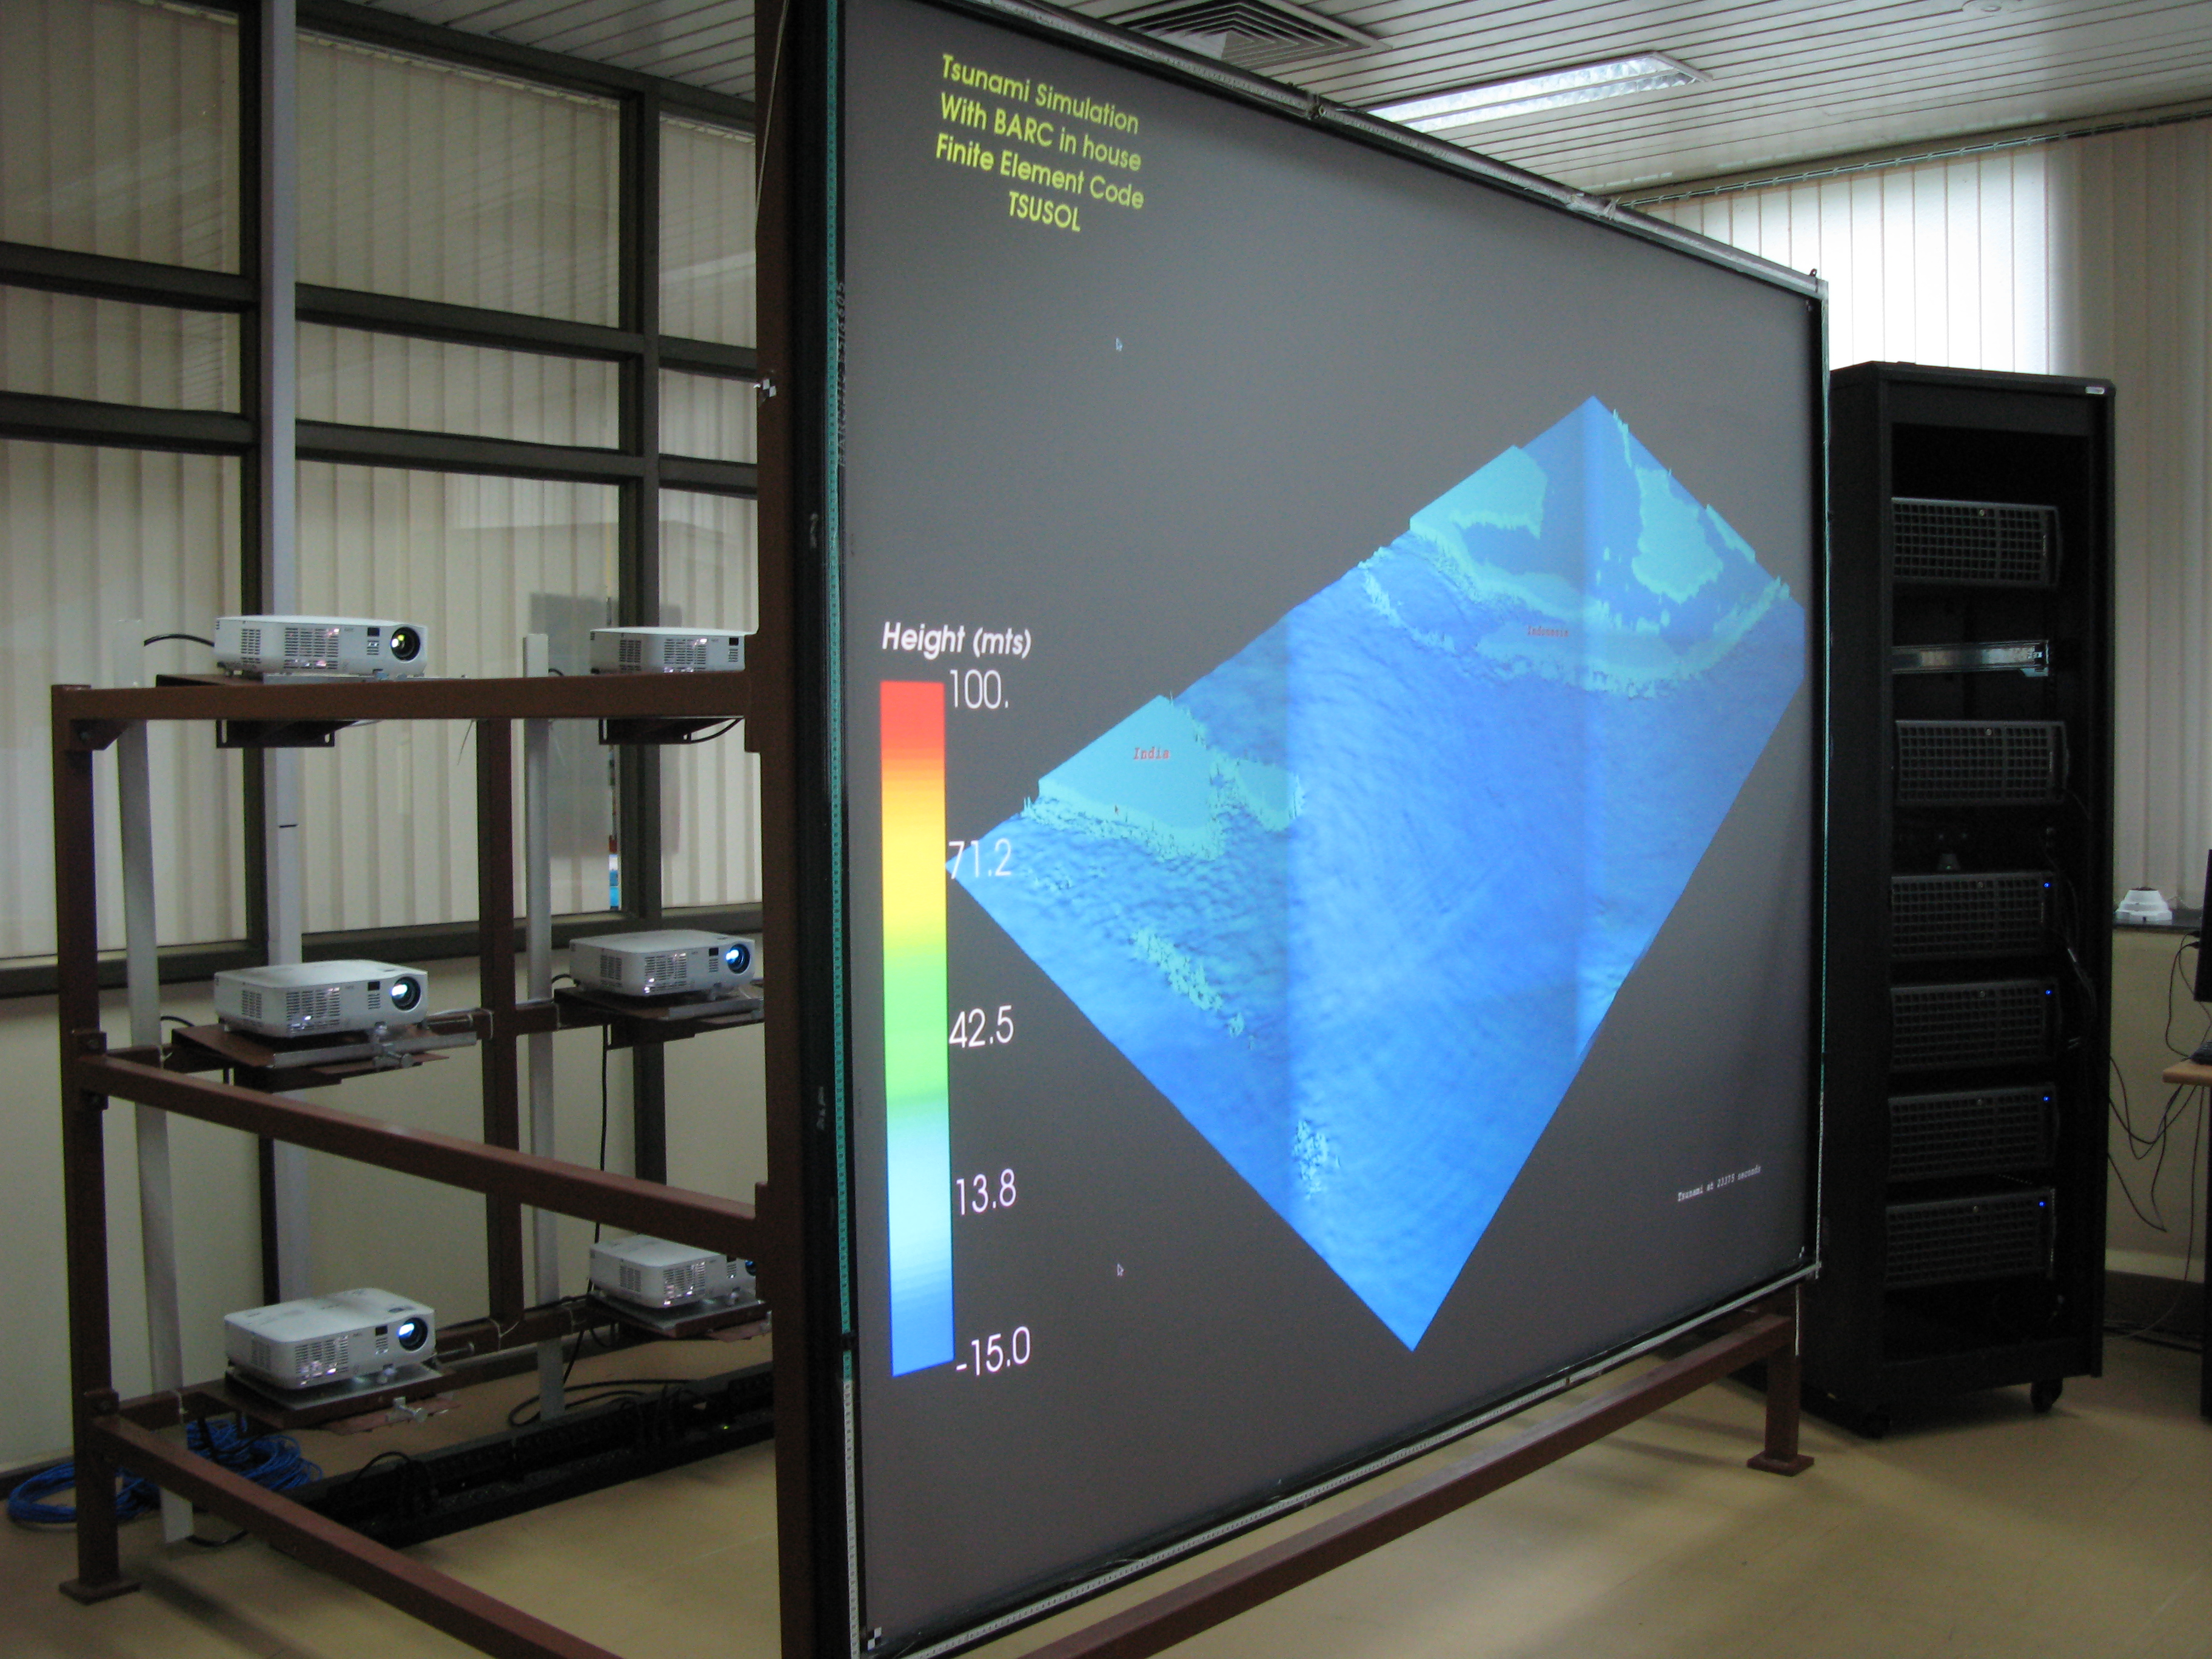
\includegraphics[width=6.0cm,height=4cm]{figures/system_setup.jpg}
\caption{Multiprojector tiled display}
\end{figure}

\end{frame}
%//////////////////////////////////////////////////////////////////////////////////////////////////////////////////////////////////

%//////////////////////////////////////////////////////////////////////////////////////////////////////////////////////////////////
\section{Motivation}
\begin{frame}
\frametitle{Motivation}
\begin{itemize}
\item Why \textit{Tiled}?
\begin{itemize}
\item Covering wider field-of-view
\item  Spatially streching high resolution content\newline
\end{itemize}
\item Why \textit{Projectors}?
\begin{itemize}
\item No bezels
\item Variable tile sizes
\end{itemize}
\end{itemize}
\end{frame}

%//////////////////////////////////////////////////////////////////////////////////////////////////////////////////////////////////
\section{Challenges}
\begin{frame}{Challenges}
\begin{enumerate}
\item Perspective distortion removal:
\begin{figure}
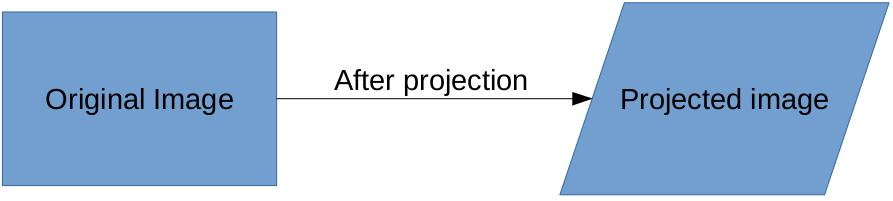
\includegraphics[width=10cm,height=2.5cm]{figures/distortion_prob.jpg}
\end{figure} 
\item Geometric continuity of projected content:
\begin{figure}
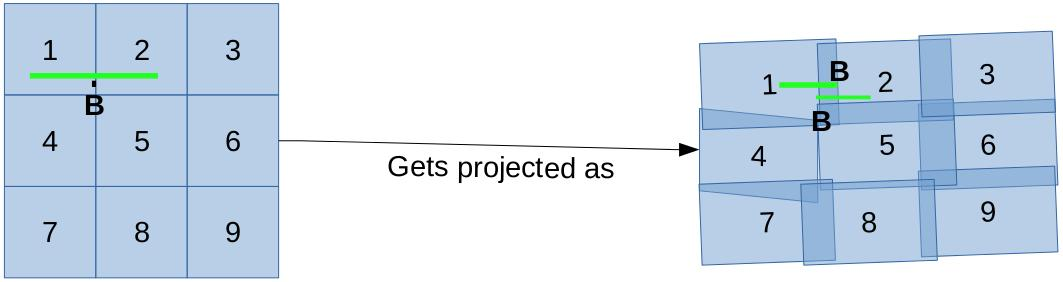
\includegraphics[width=10cm, height=2.5cm]{figures/continuity_prob.jpg}
\end{figure}
\item Handling intensity in overlap region:
\end{enumerate}
\end{frame}

%//////////////////////////////////////////////////////////////////////////////////////////////////////////////////////////////////
\section{Followed approach}
\begin{frame}{Followed approach}
\begin{itemize}
\item Removing perspective distortion:
\begin{figure}
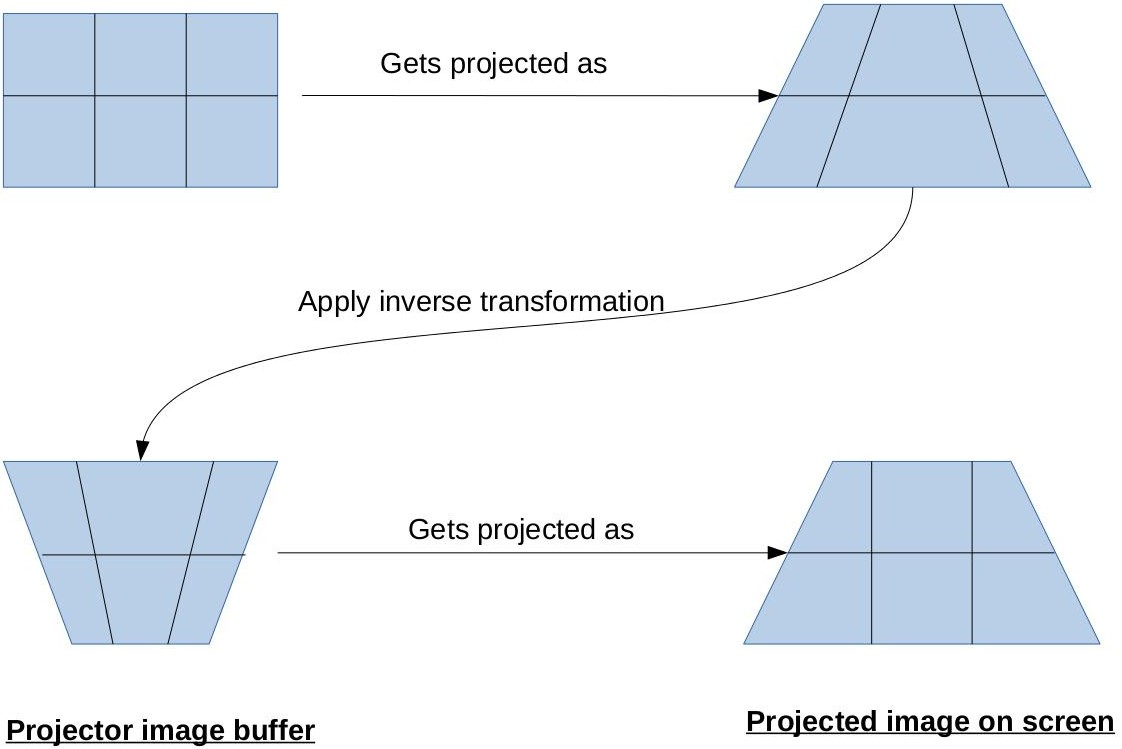
\includegraphics[width=7cm, height=5cm]{figures/distort_sol.jpg}
\end{figure}
\end{itemize}
\end{frame}

%//////////////////////////////////////////////////////////////////////////////////////////////////////////////////////////////////

\begin{frame}{Followed approach(contd.)}
\begin{itemize}
\item Ensuring geometric continuity:
\begin{figure}
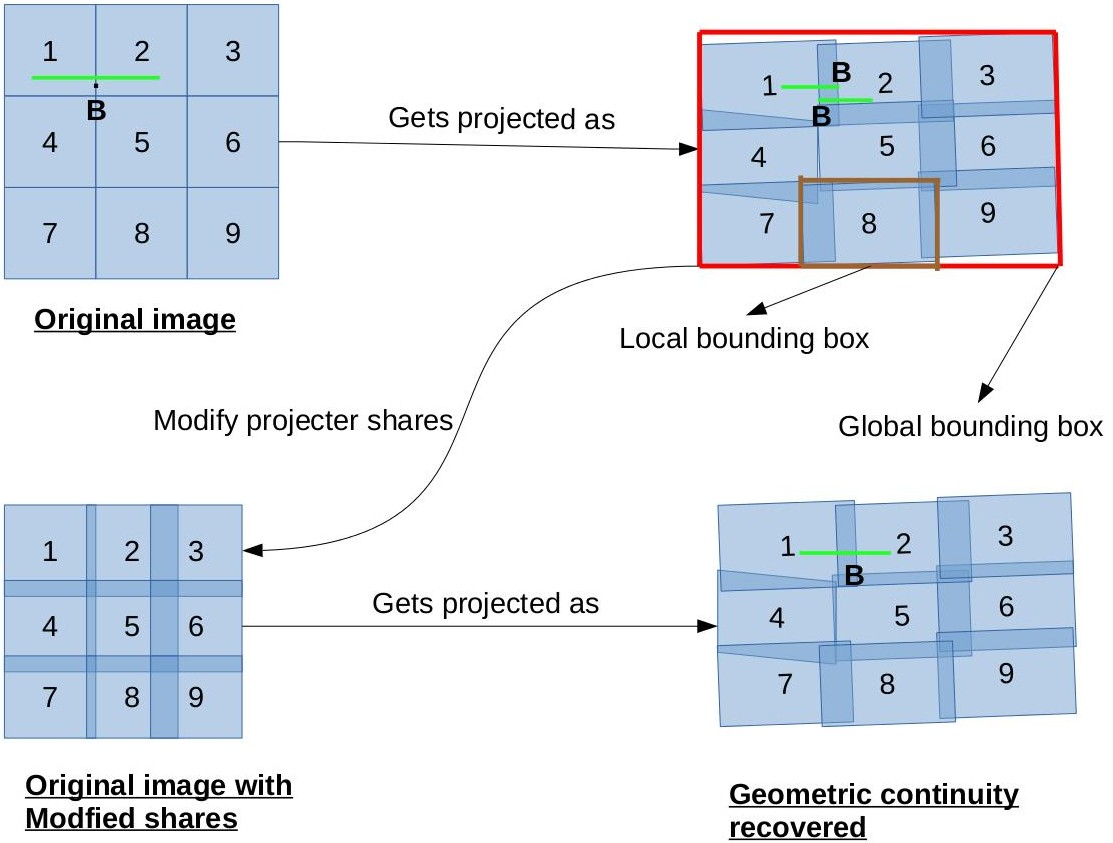
\includegraphics[width=8cm,height=6cm]{figures/continuity_better.jpg}
\end{figure}
\end{itemize}
\end{frame}


%//////////////////////////////////////////////////////////////////////////////////////////////////////////////////////////////////

\begin{frame}{Followed approach(contd.)}
\begin{itemize}
\item Handling image intensity at the overlap region:
\begin{figure}
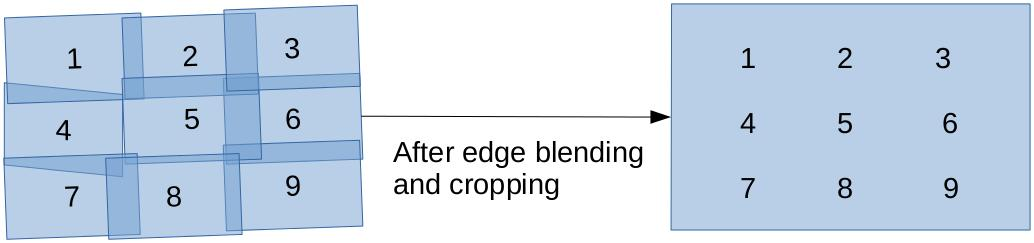
\includegraphics[width=9cm,height=3cm]{figures/blending.jpg}
\end{figure}
\end{itemize}
\end{frame}

%//////////////////////////////////////////////////////////////////////////////////////////////////////////////////////////////////

\section{System setup}
\begin{frame}
\frametitle{System setup}
Developed system has:
\begin{itemize}
\item 3X3 grid of projectors
\item Rear projection screen
\item 1 digital camera
\item Workstations arranged in master-slave configuration
\end{itemize}

\begin{figure}
\centering
\begin{tabularx}{\linewidth}{@{}cXX@{}}
\begin{tabular}{c c}
\hspace{0.5cm}\subfloat[System setup]{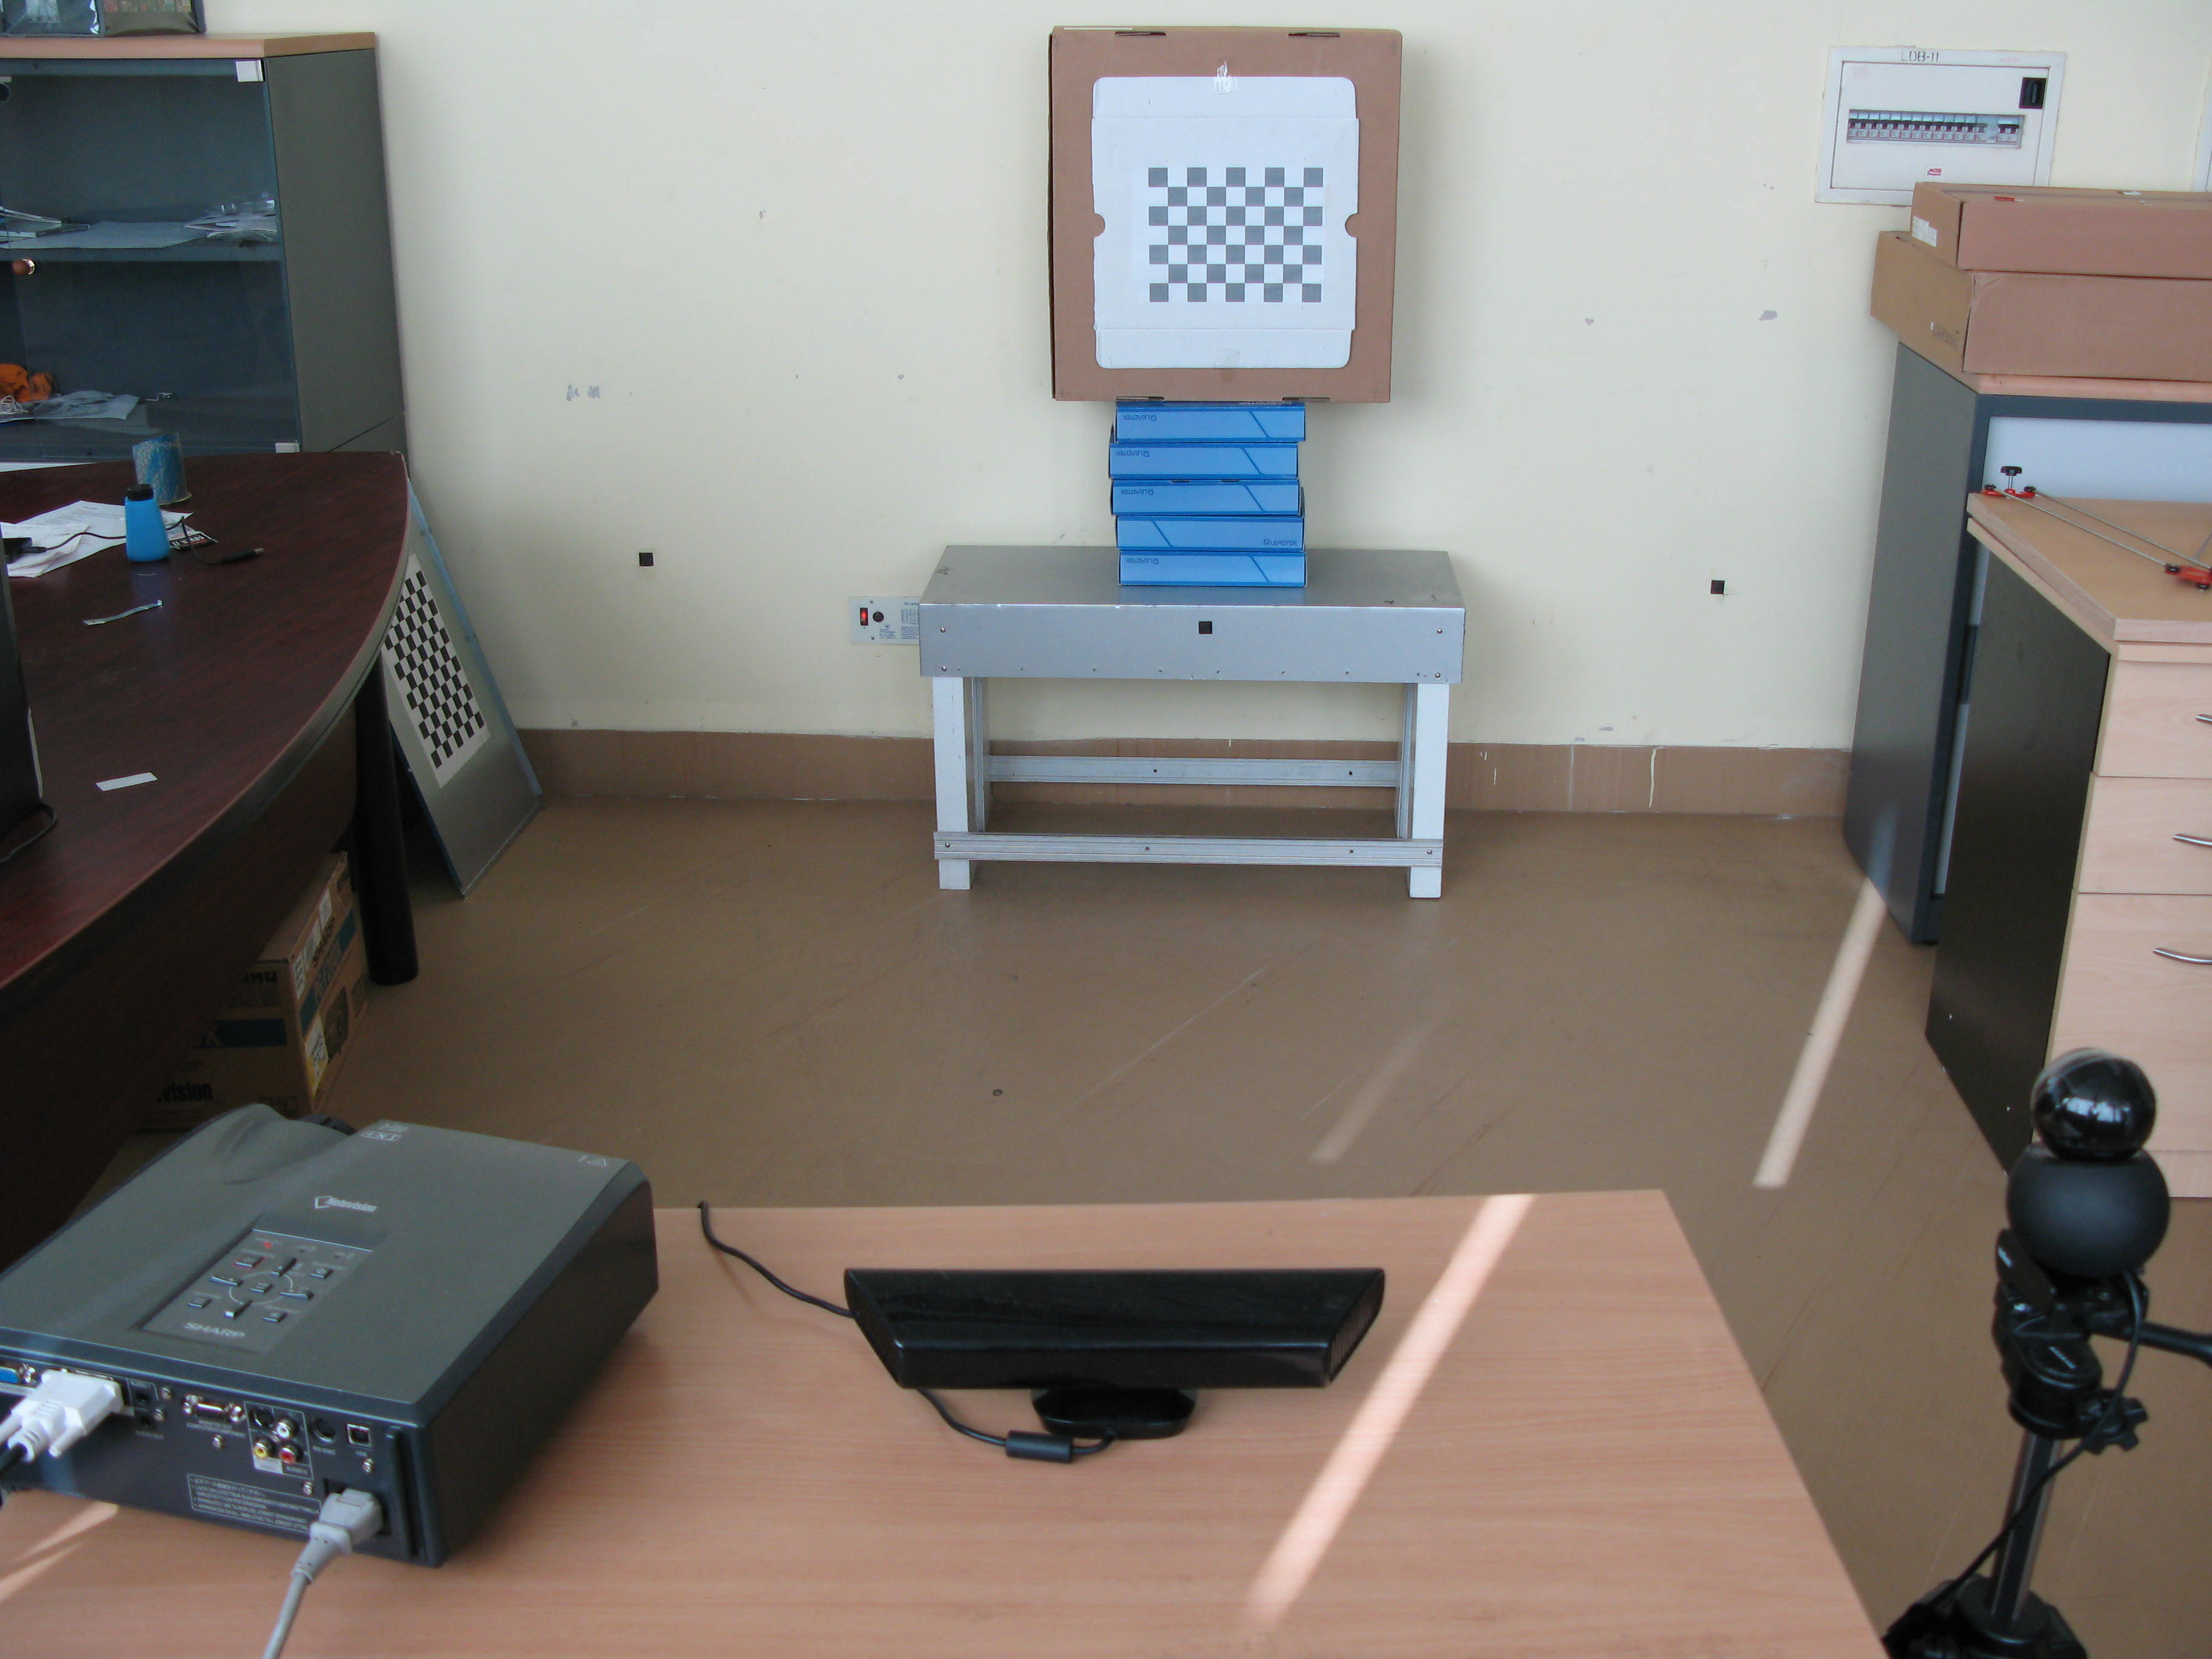
\includegraphics[width=4.5cm,height=3cm]{figures/setup.jpg}} & 
\subfloat[Projector-array behind the projection screen]{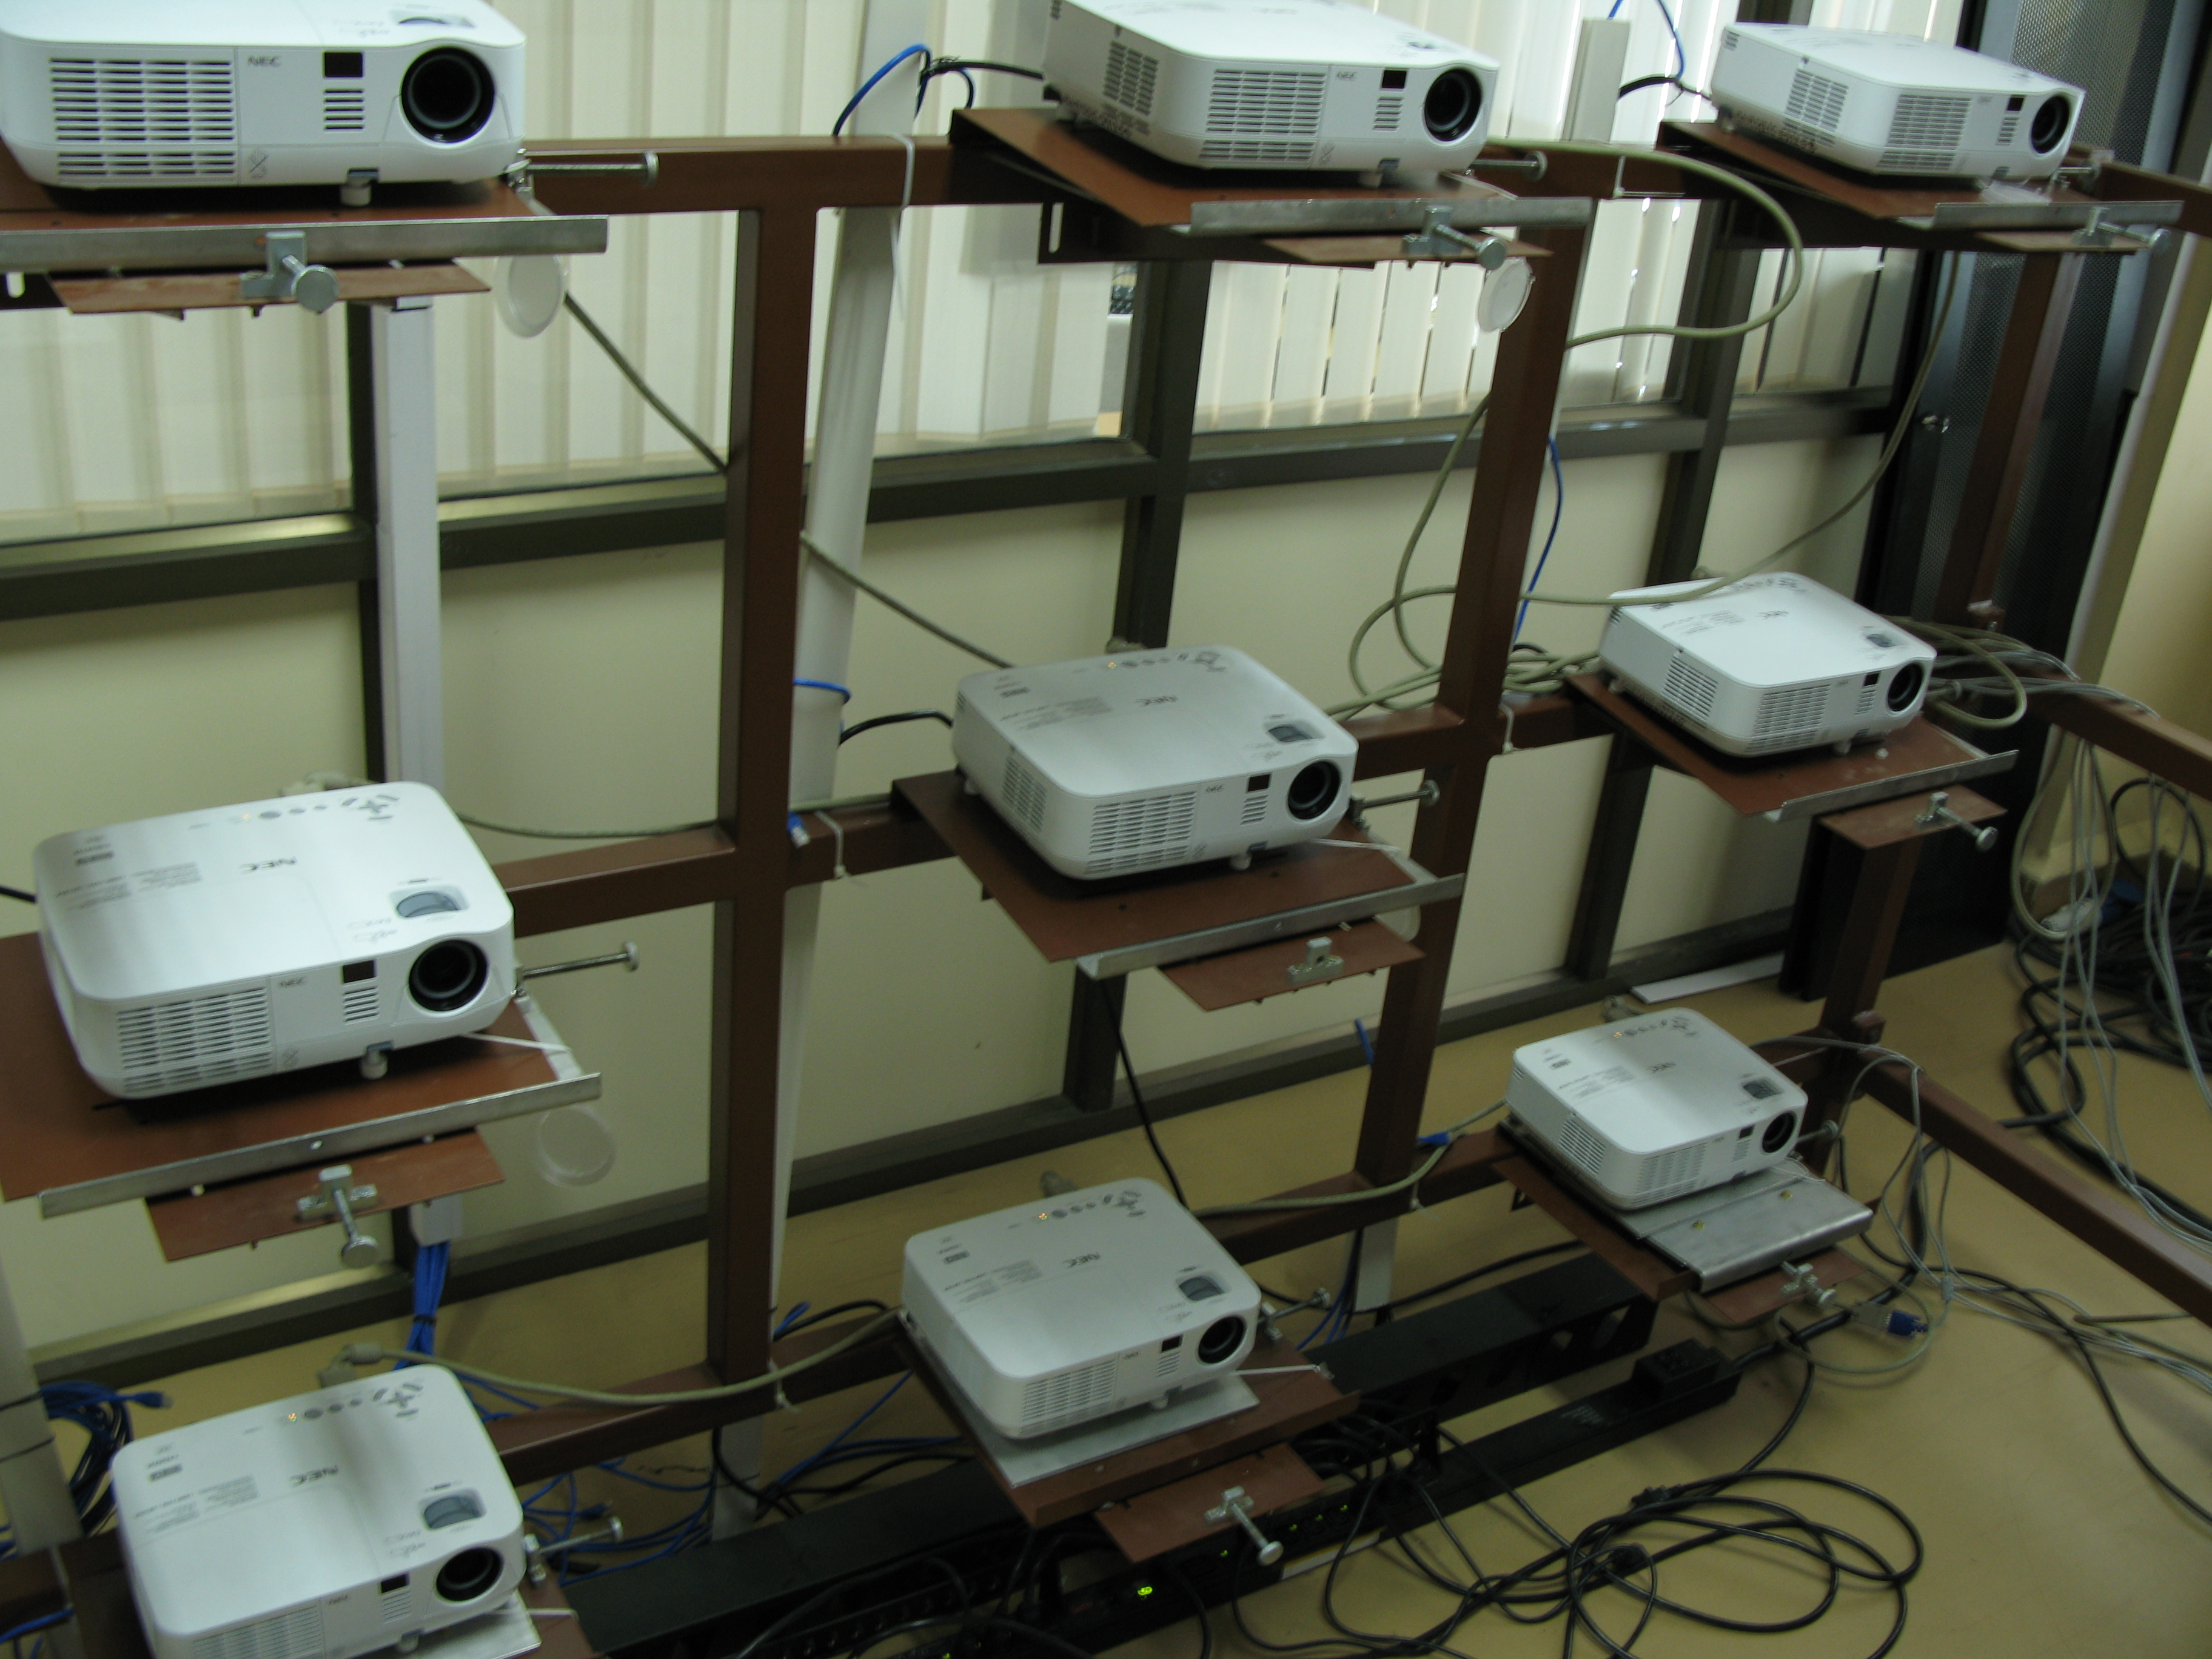
\includegraphics[width=4.5cm,height=3cm]{figures/projs.jpg}} \\
\end{tabular}
\end{tabularx}
\end{figure}

\end{frame}

%//////////////////////////////////////////////////////////////////////////////////////////////////////////////////////////////////
\section{Algorithm}
\begin{frame}{Algorithm}
\begin{itemize}
\item Based on paper `A practical and flexible tiled
display system' by M.S. Brown and W.B. Seales.
\item \underline{Algorithm overview}:
\begin{enumerate}
\item Compute Camera-screen homograhy
\item Project and detect features(i.e., checkerboard)
\item Address detected coordinates wrt. local bounding box coordinate system 
\item Address local bounding boxes wrt. global bounding box coordinate system
\item Compute overlap between adjacent projectors
\item Attenuate intensities in overlap regions
\end{enumerate}
\end{itemize}
\end{frame}

%//////////////////////////////////////////////////////////////////////////////////////////////////////////////////////////////////

\begin{frame}
\frametitle{Algorithm(contd.)}
\framesubtitle{Compute screen to camera relation}
\begin{itemize}
\item \hyperlink{concept}{\textit{Geometrically aligned}} and \hyperlink{concept}{\textit{seamless}} content required on projection screen
\item Camera is just a \textit{feedback device}
\item All later calculations are performed in screen-coordinate system
\end{itemize}

\begin{figure}
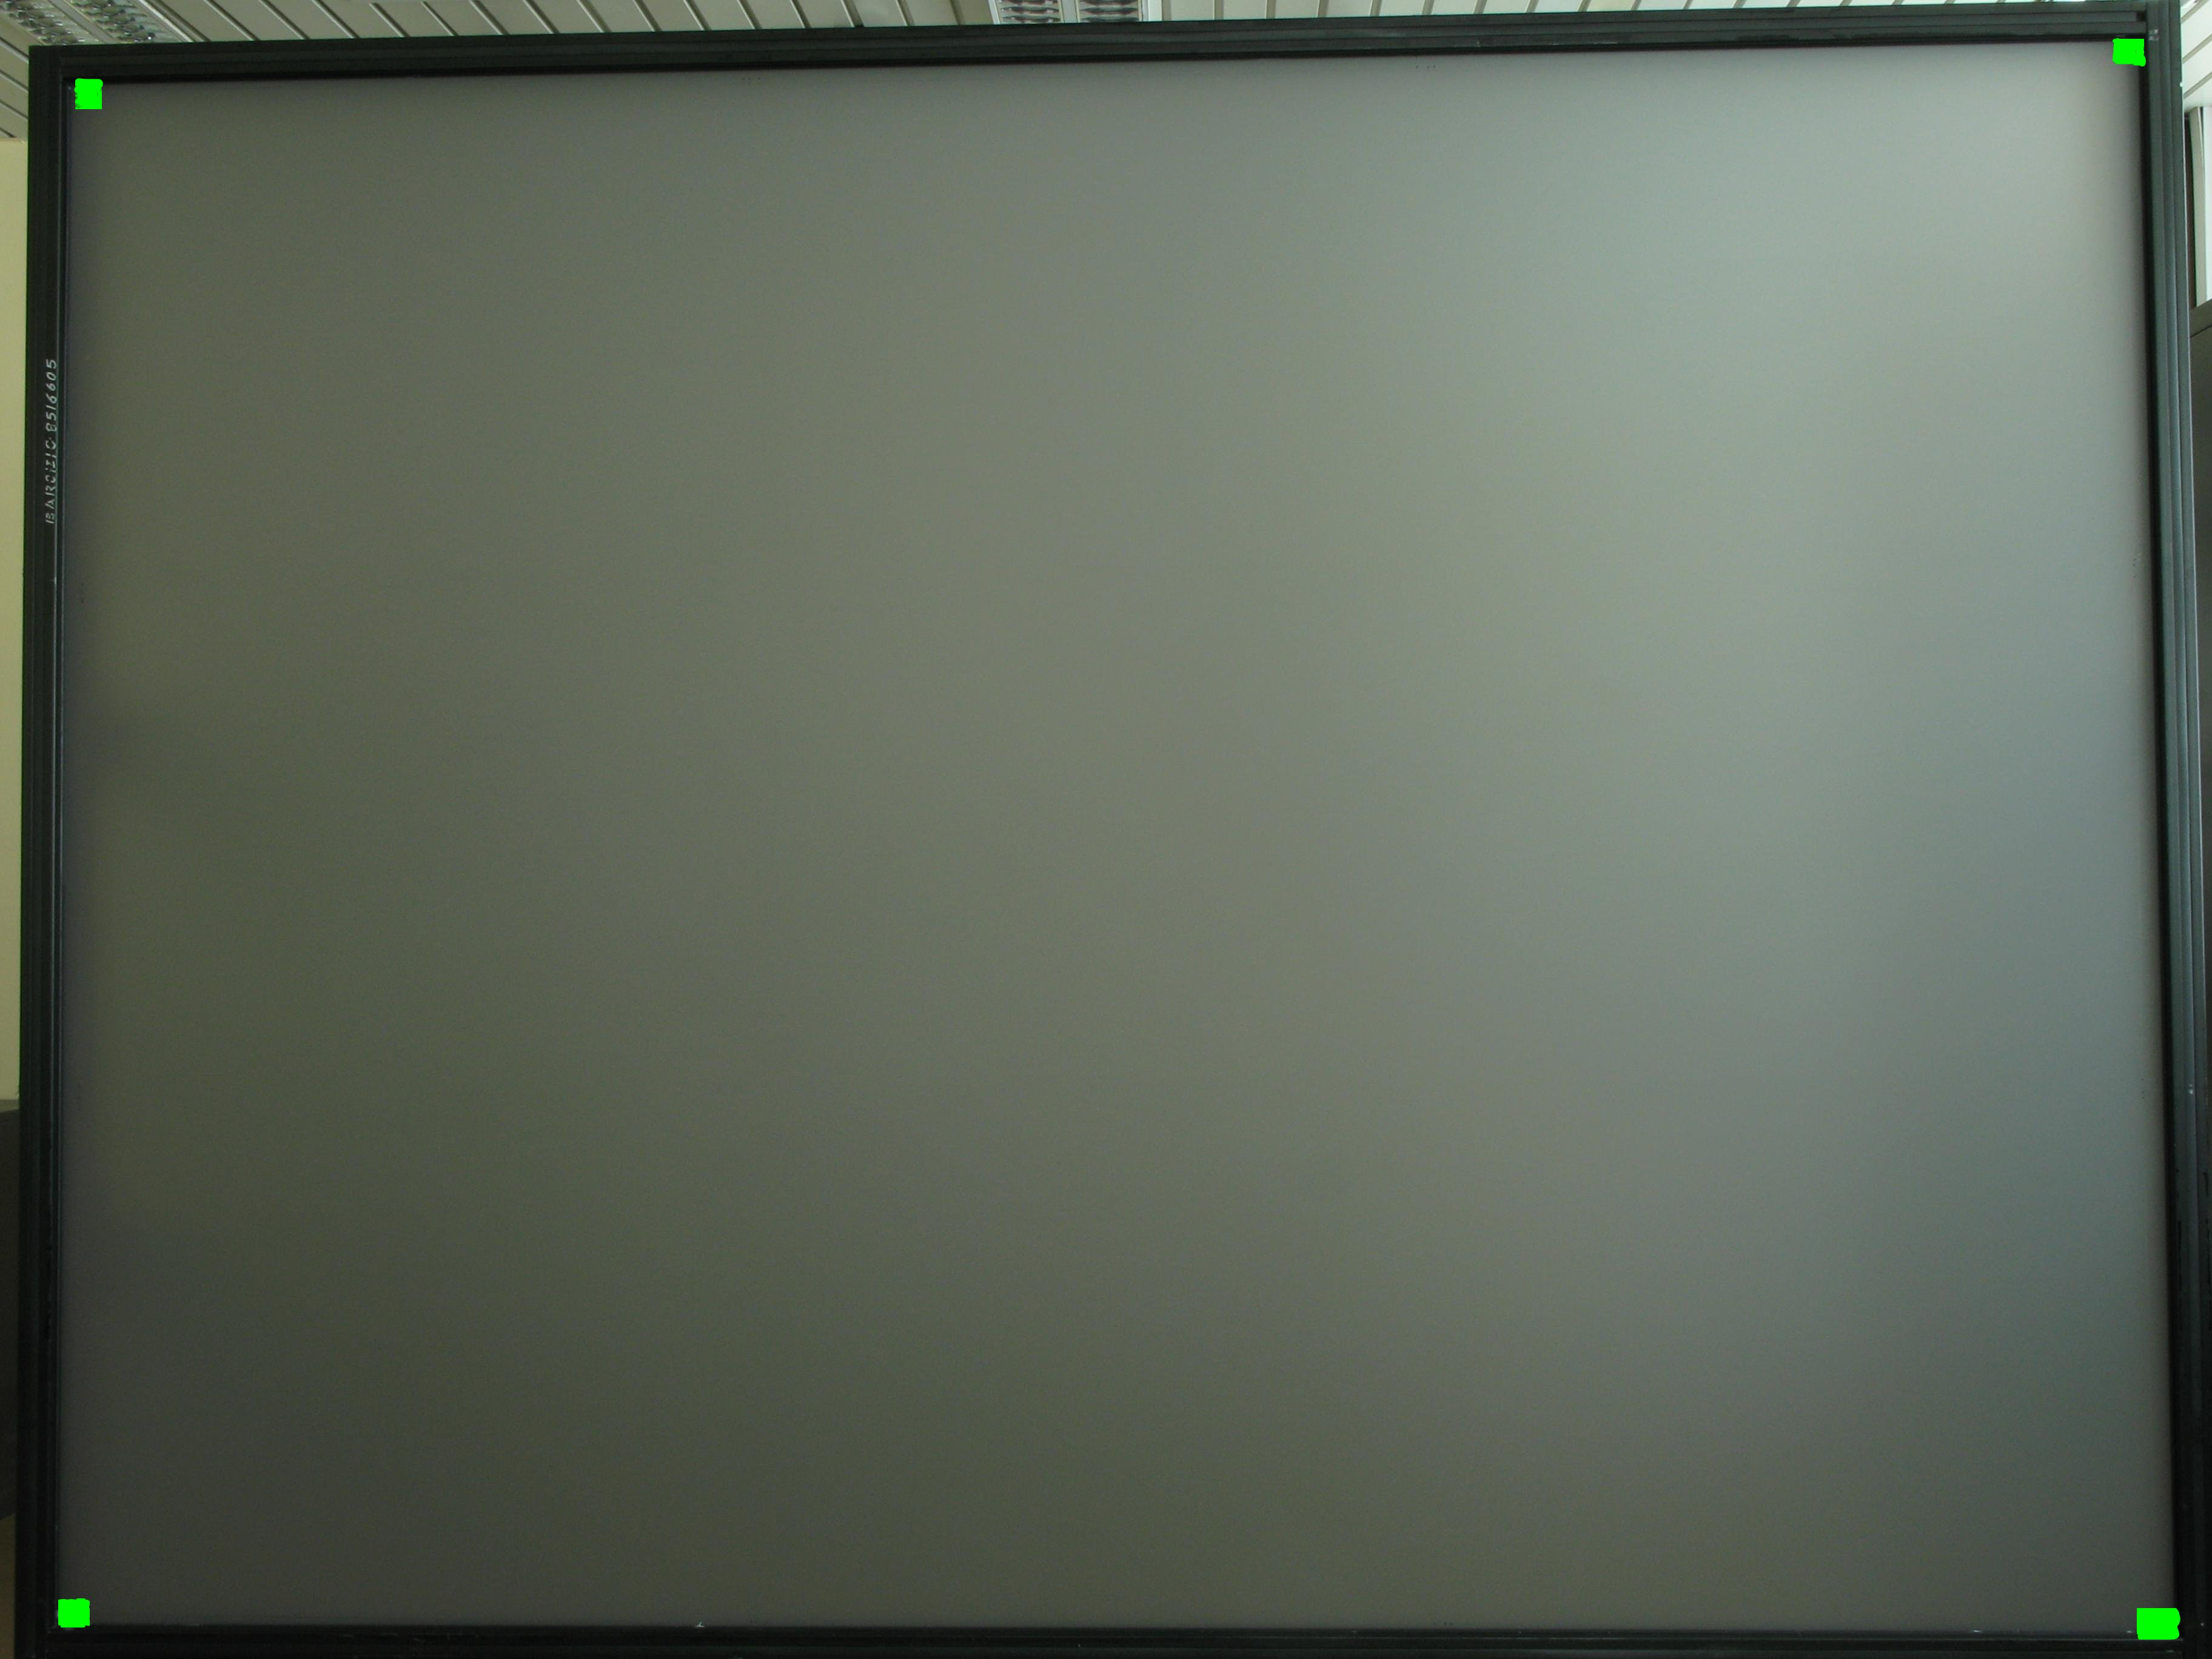
\includegraphics[width=6cm, height = 4cm]{figures/debug_image_features.jpg}
\caption{View from camera}
\end{figure}
\end{frame}

%//////////////////////////////////////////////////////////////////////////////////////////////////////////////////////////////////

\begin{frame}
\frametitle{Algorithm(contd.): Remove perspective distortion}
\framesubtitle{Project and detect features for each projector}
\begin{itemize}
\item Detected features are mapped to screen coordinate system
\end{itemize}

\begin{figure}
\centering
\begin{tabularx}{\linewidth}{@{}cXX@{}}
\begin{tabular}{c c}
\hspace{0.5cm}\subfloat[Projected features]{
\includegraphics[width=4.5cm,height=3cm]{figures/checkerboard.jpg}} &
\subfloat[Low exposure image of detected features for the central projector]{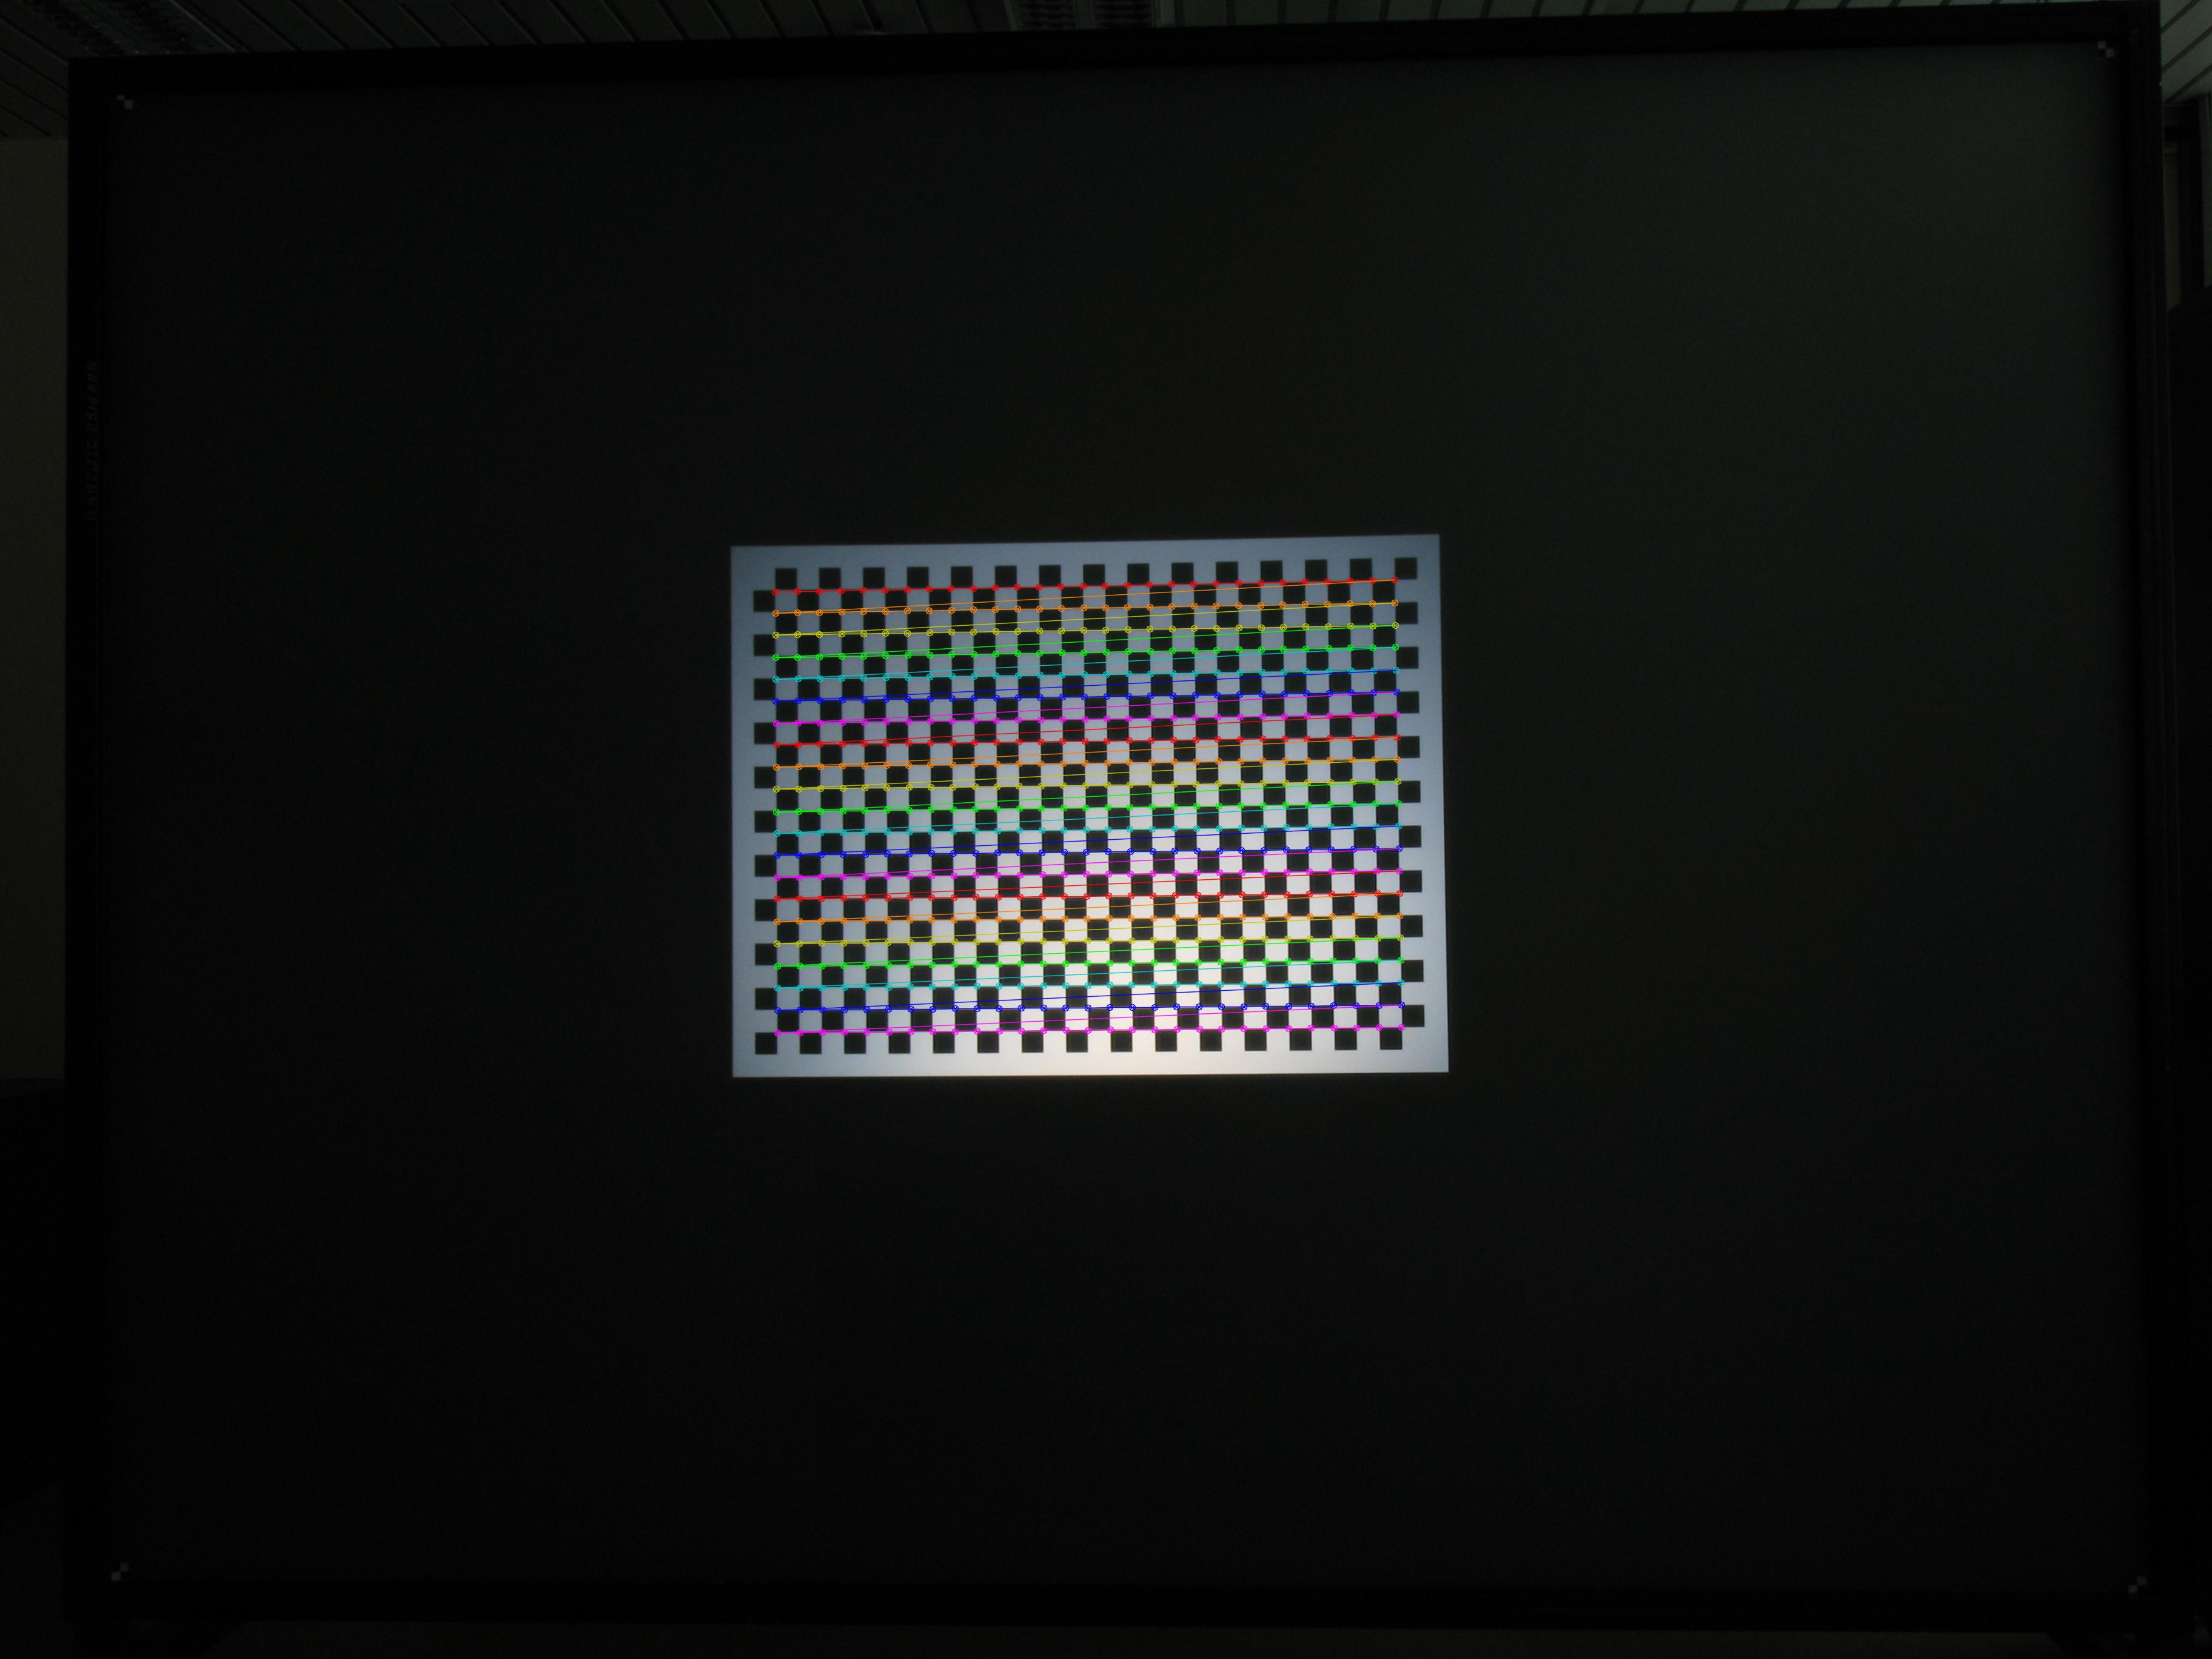
\includegraphics[width=6cm, height=4cm]{figures/detected_corners.jpg}} \\
\end{tabular}
\end{tabularx}
\end{figure}

\end{frame}

%//////////////////////////////////////////////////////////////////////////////////////////////////////////////////////////////////

\begin{frame}
\frametitle{Algorithm(contd.): Remove perspective distortion}
\framesubtitle{Compute \textit{local} bounding boxes}
\begin{itemize}
\item Compute normalized pair of $(coordinate_{\textit{original image}}, coordinate_{\textit{detected}})$ for each checkerboard corner.
\end{itemize}

\begin{figure}
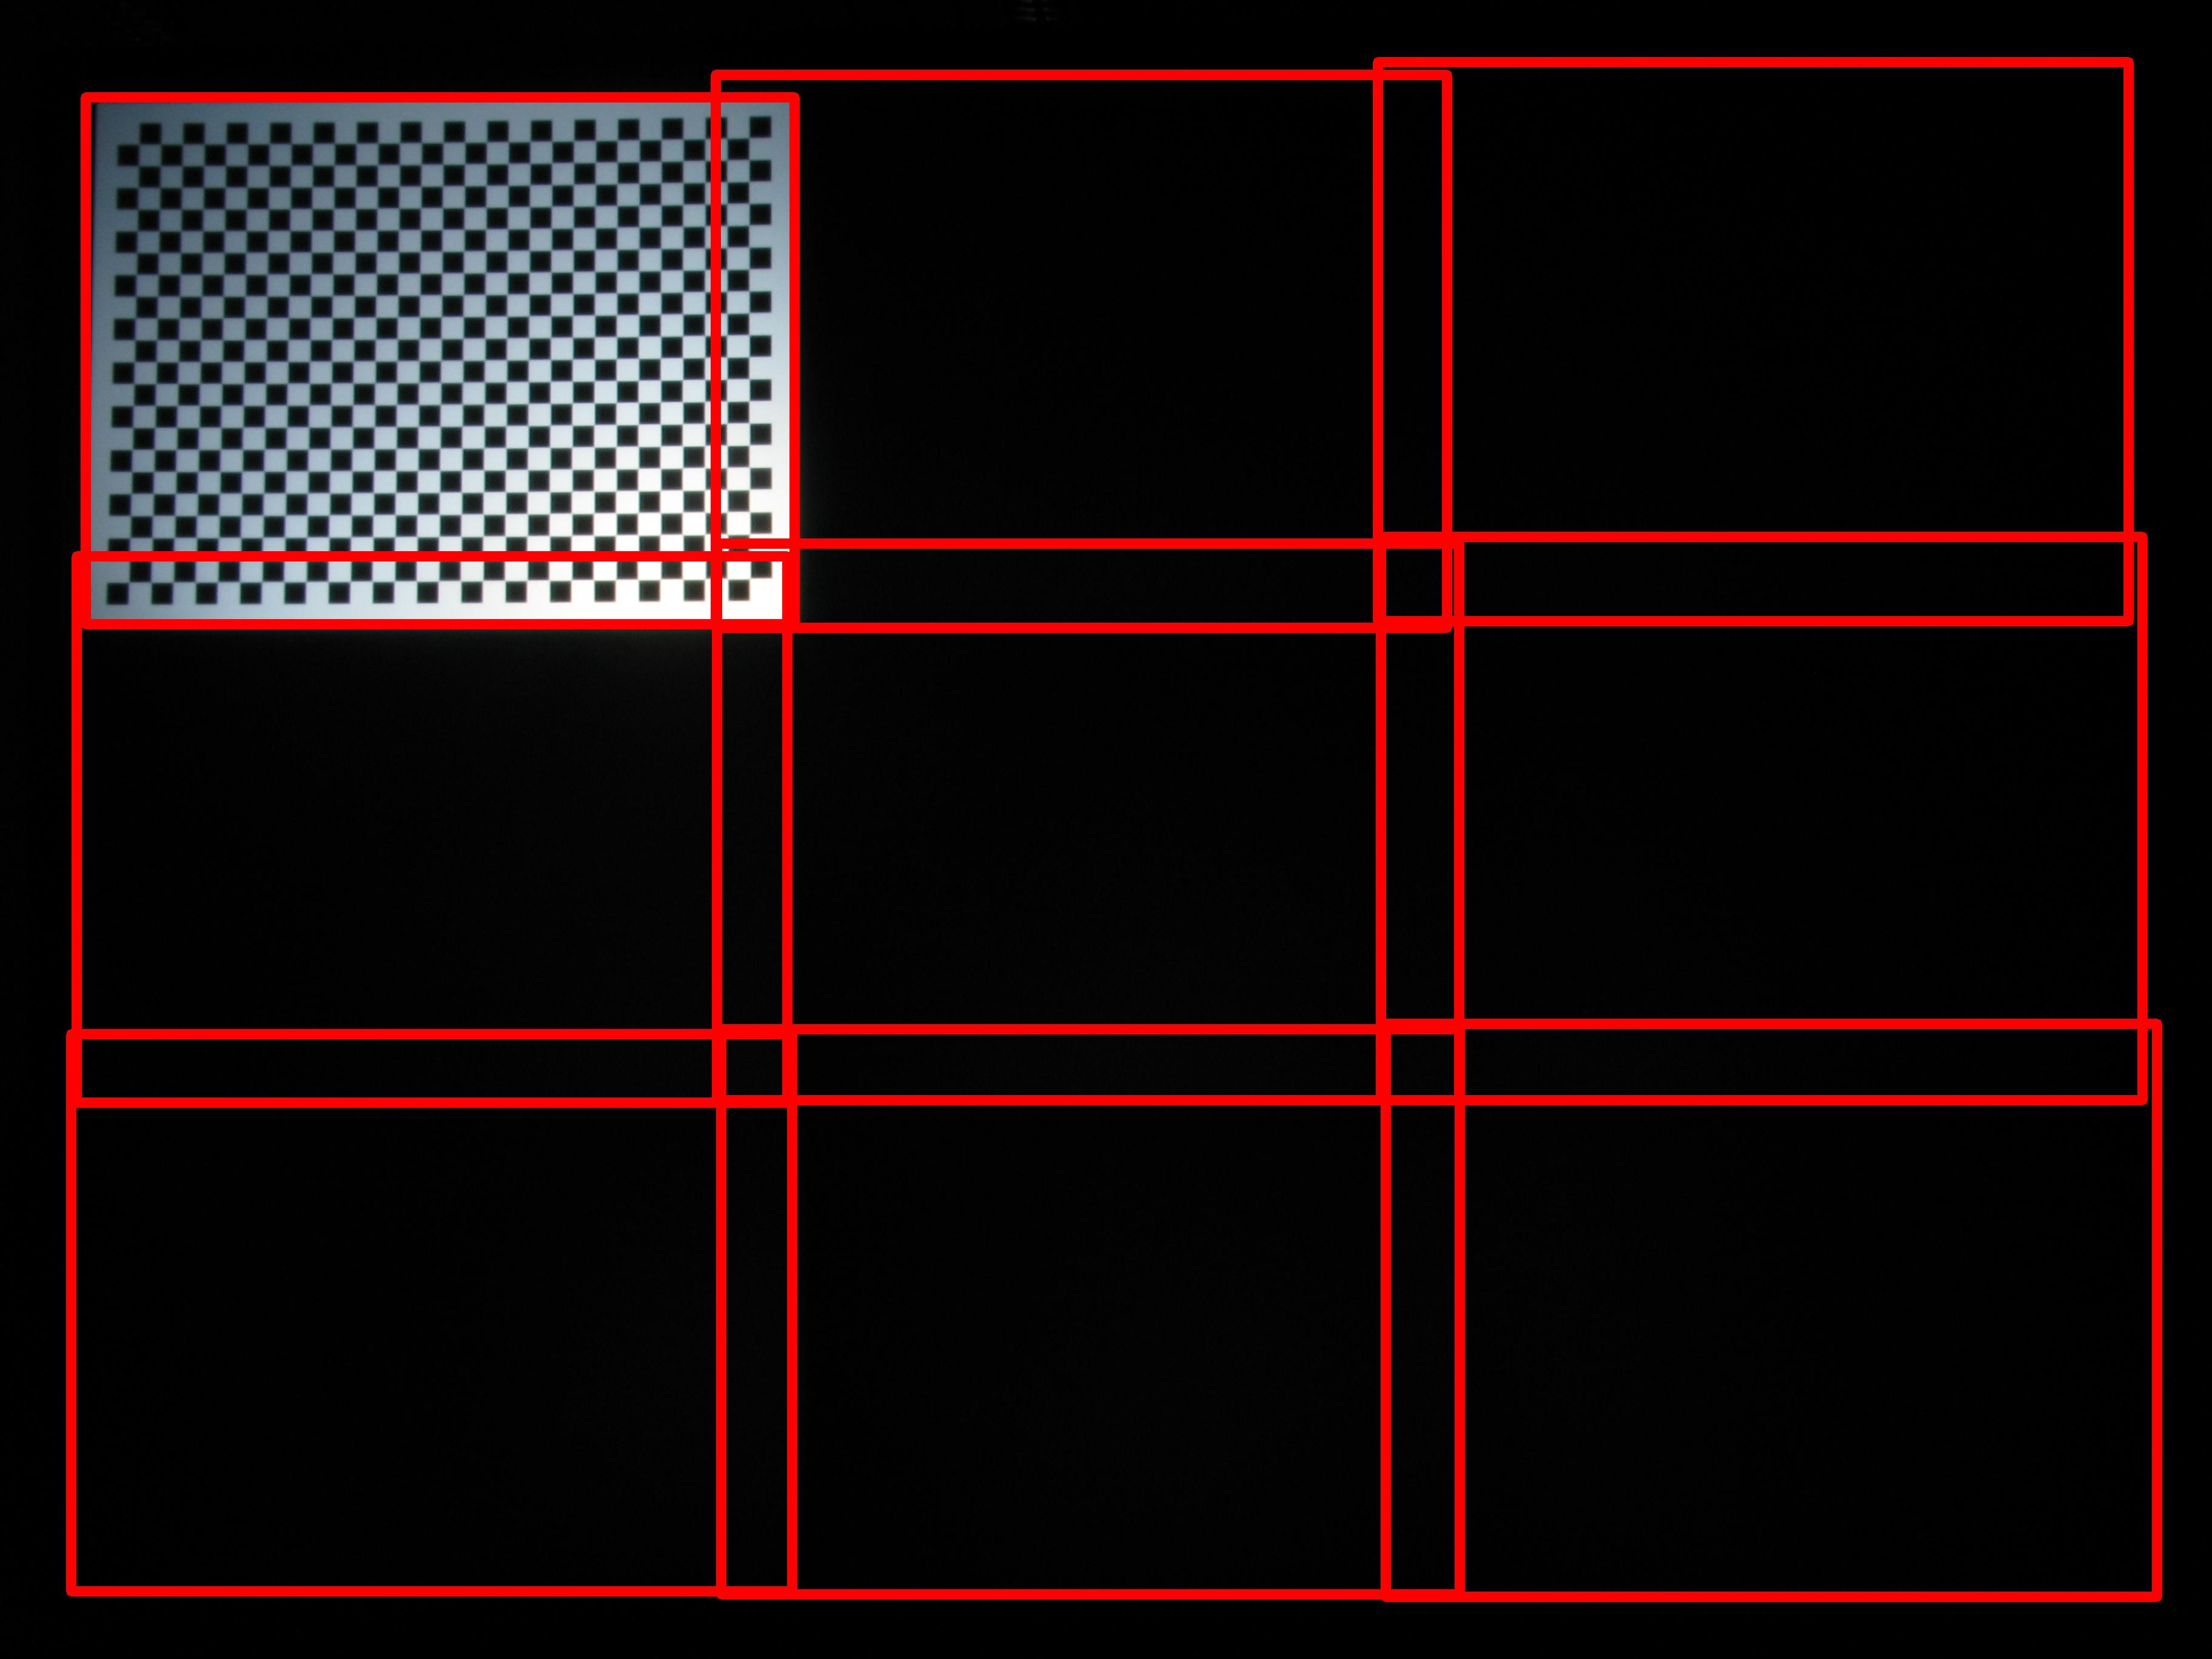
\includegraphics[width=6cm,height=4cm]{figures/all_bboxes.jpg}
\caption{Boxes bounding the projection region of each projector}
\end{figure}

\end{frame}

%//////////////////////////////////////////////////////////////////////////////////////////////////////////////////////////////////

\begin{frame}
\frametitle{Algorithm(contd.): Geometric continuity}
\framesubtitle{Compute \textit{global} bounding box}
\begin{itemize}
\item Addressing all local bounding boxes wrt. a common coordinate system. 
\item Global bounding box represents the original image to projected on the screen.
\item Helps in computing share of each projector in the original image.
\end{itemize}

\begin{figure}
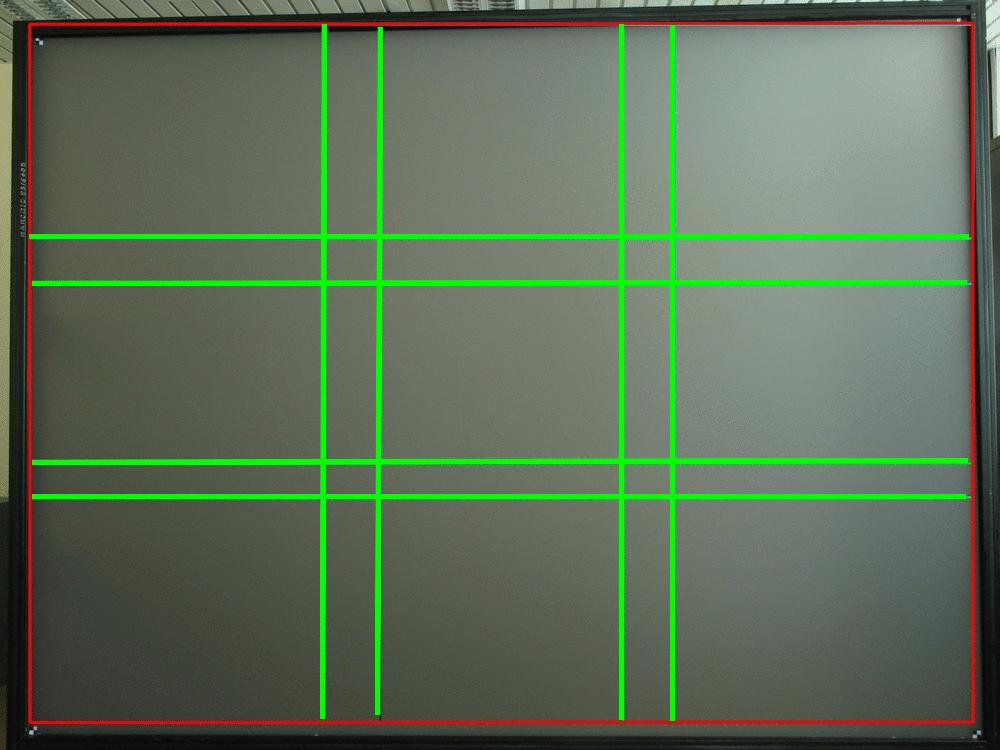
\includegraphics[width=6cm,height=4cm]{figures/test.jpg}
\end{figure}
\end{frame}

%//////////////////////////////////////////////////////////////////////////////////////////////////////////////////////////////////

\begin{frame}
\frametitle{Algorithm(contd.): Seamlessness}
\framesubtitle{Compute alpha-map\textsuperscript{\hyperlink{distform}{*}}}
\begin{enumerate}
\item Compute \hyperlink{concept}{region of overlap} between adjacent projectors.
\item Attenuate image intensity of each overlapping projector.
\end{enumerate}

\begin{figure}
\centering
\begin{tabularx}{\linewidth}{@{}cXX@{}}
\begin{tabular}{c c}
\hspace{0.5cm}\subfloat[Projection region]{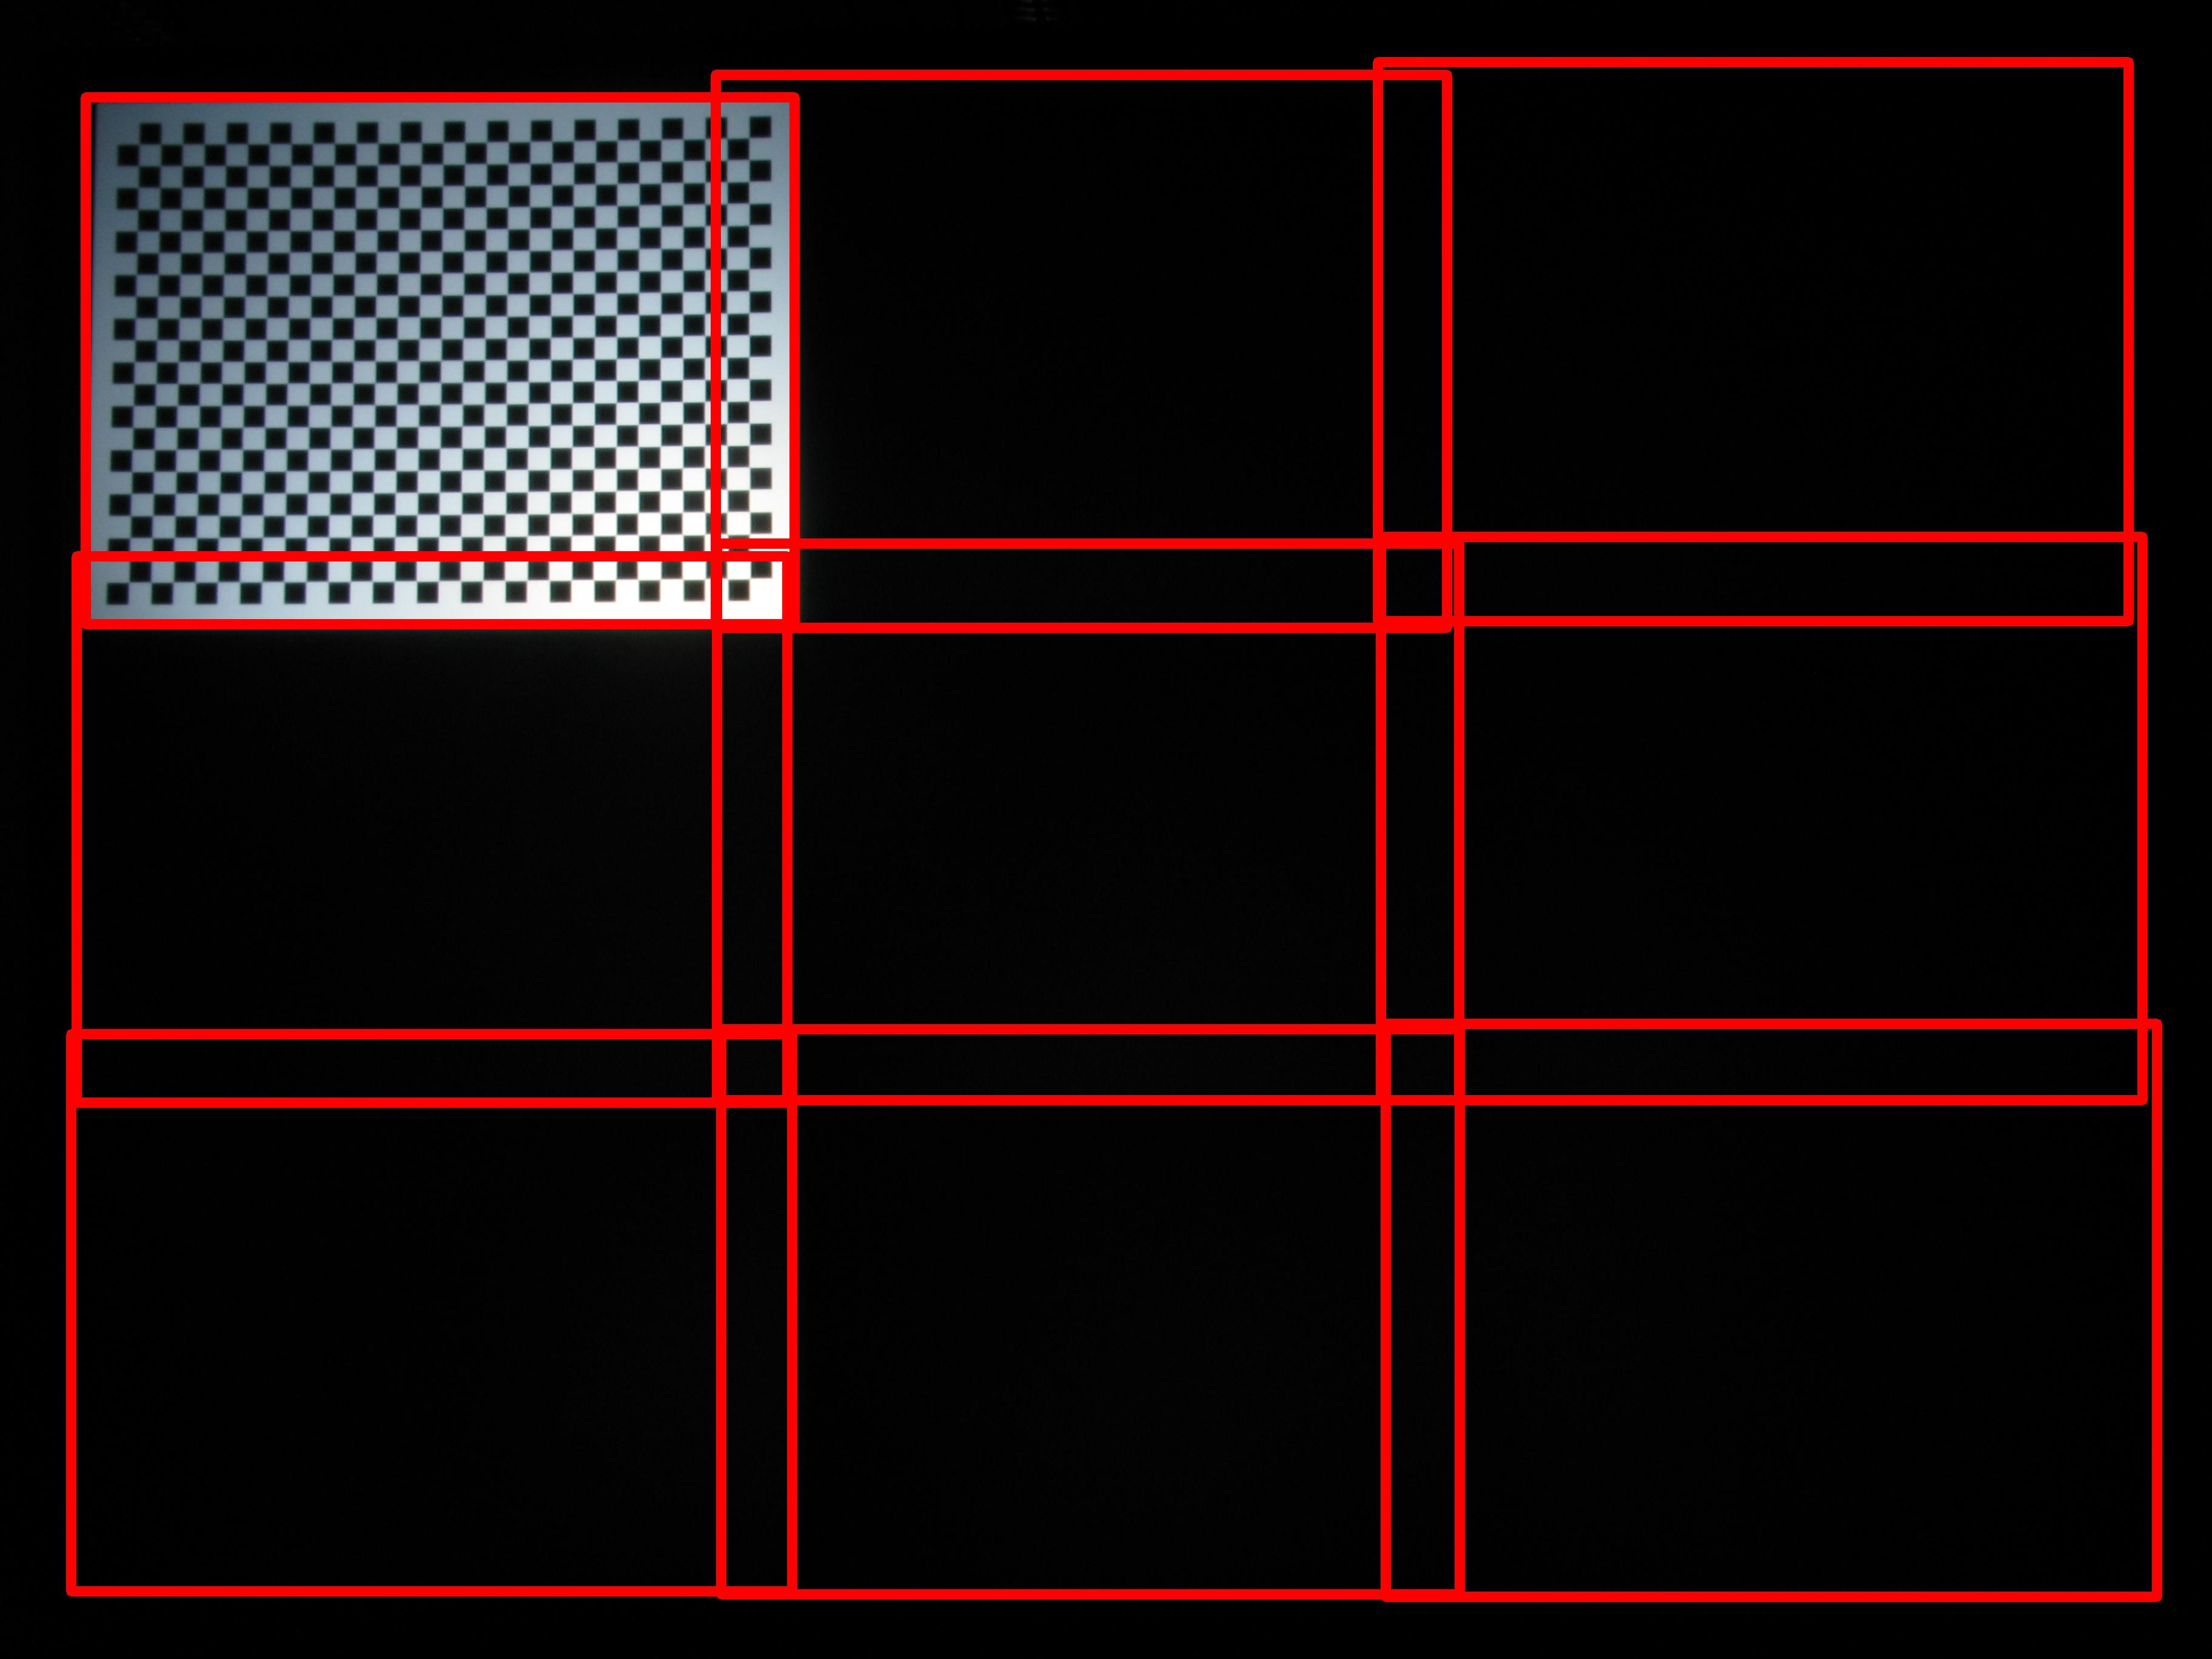
\includegraphics[width=4.5cm,height=3cm]{figures/all_bboxes.jpg}} &
\subfloat[Corresponding attenuation map]{
\includegraphics[width=4.5cm,height=3cm]{figures/alpha_map_6.jpg}} \\
\end{tabular}
\end{tabularx}
\end{figure}

\end{frame}

%//////////////////////////////////////////////////////////////////////////////////////////////////////////////////////////////////
\section{Contributions}
\begin{frame}
\frametitle{Contributions}
\underline{Corrected detected corners using line fitting}:
\begin{itemize}
\item Utilized the fact that collinearity under perspective projection is preserved
\item Fitted line on detected corners and corrected the detected coordinates using intersection of fitted lines
\item Resulted in more uniform texture mapping
\end{itemize}

\begin{figure}
\centering
\begin{tabularx}{\linewidth}{@{}cXX@{}}
\begin{tabular}{c c}
\hspace{0.5cm}\subfloat[Without line fitting]{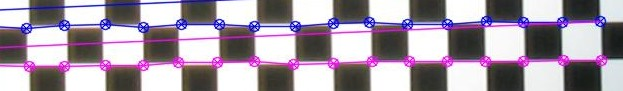
\includegraphics[width=4.5cm,height=1.0cm]{figures/test1.jpg}} & 
\subfloat[With line fitting]{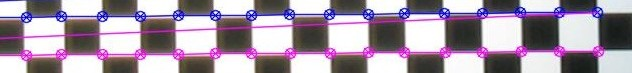
\includegraphics[width=4.5cm,height=1.0cm]{figures/test2.jpg}} \\
\end{tabular}
\end{tabularx}
\end{figure}

\end{frame}

%//////////////////////////////////////////////////////////////////////////////////////////////////////////////////////////////////

\begin{frame}{Contributions(contd.)}

\underline{Used Cross-ratio\textsuperscript{\hyperlink{crossrat}{*}} invariant to recover full projection region}:

\begin{itemize}
\item It is a perspective projection invariant
\item Relates 4 collinear points:
$CR_p=\frac{|AC|_c*|BD|_c}{|BC|_c*|AD|_c}$
\end{itemize}

\begin{figure}
\centering
\begin{tabularx}{\linewidth}{@{}cXX@{}}
\begin{tabular}{c c}
\subfloat[Applying cross ratio invariant]{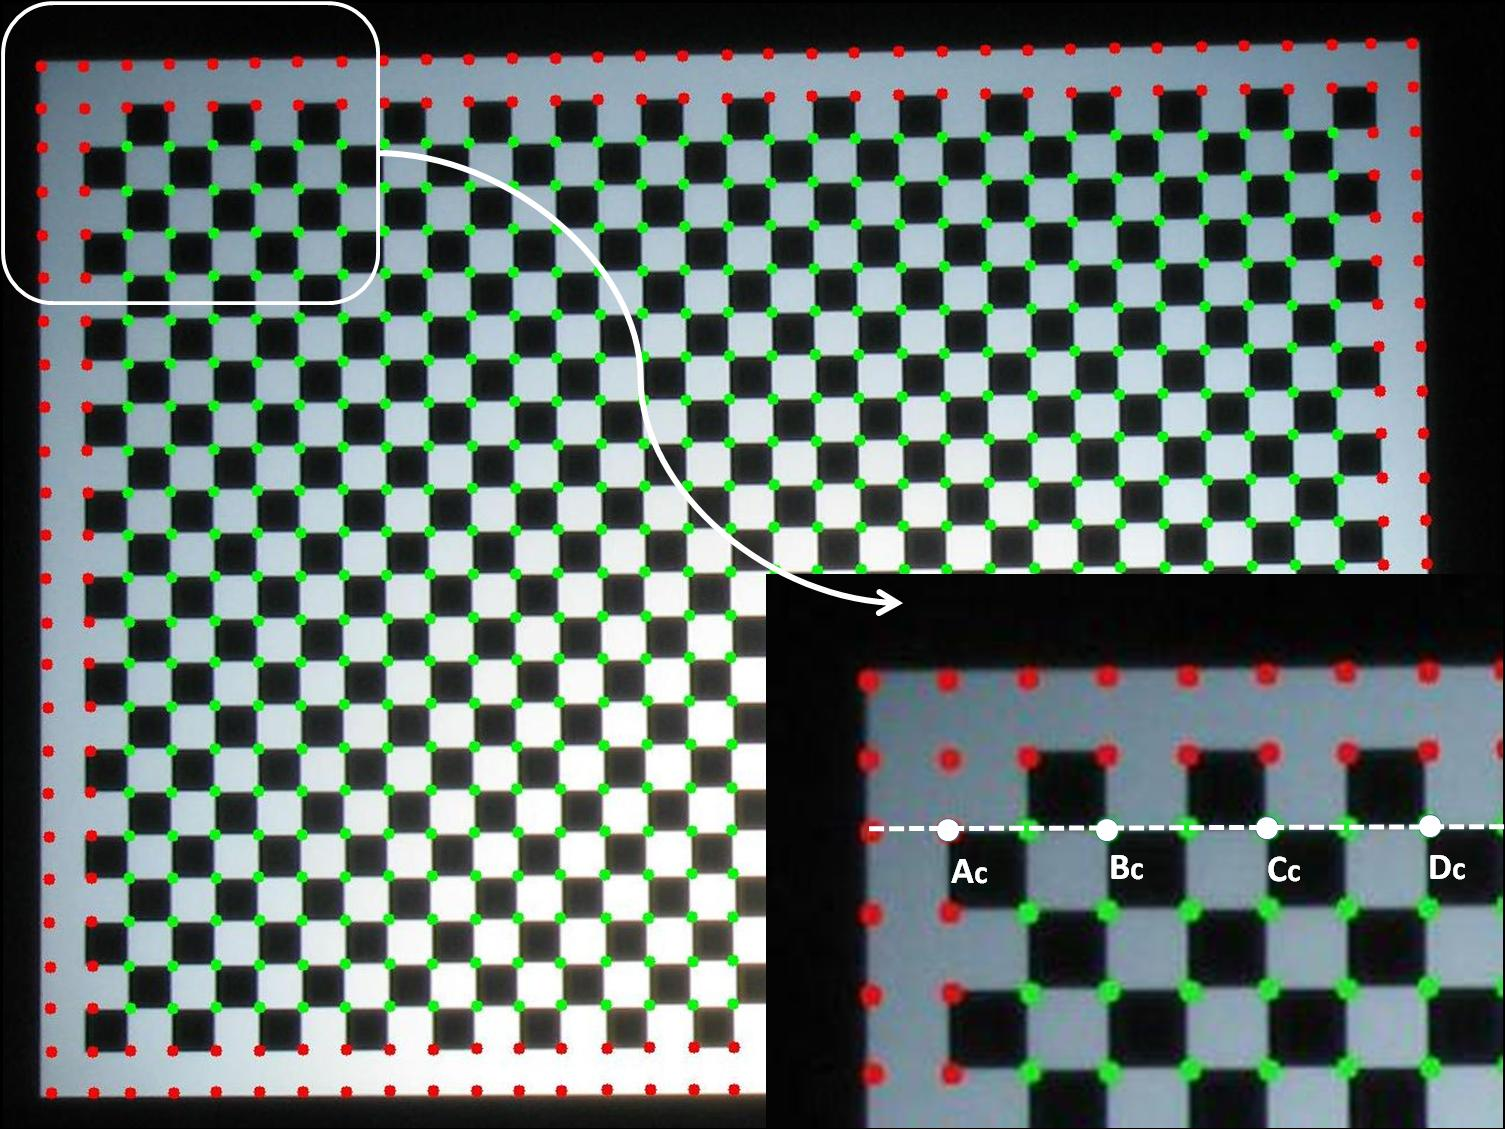
\includegraphics[width=5.0cm,height=4.0cm]{figures/cross_rat_img.jpg}} &
\subfloat[green: without cross ratio, blue: with cross ratio invariant]{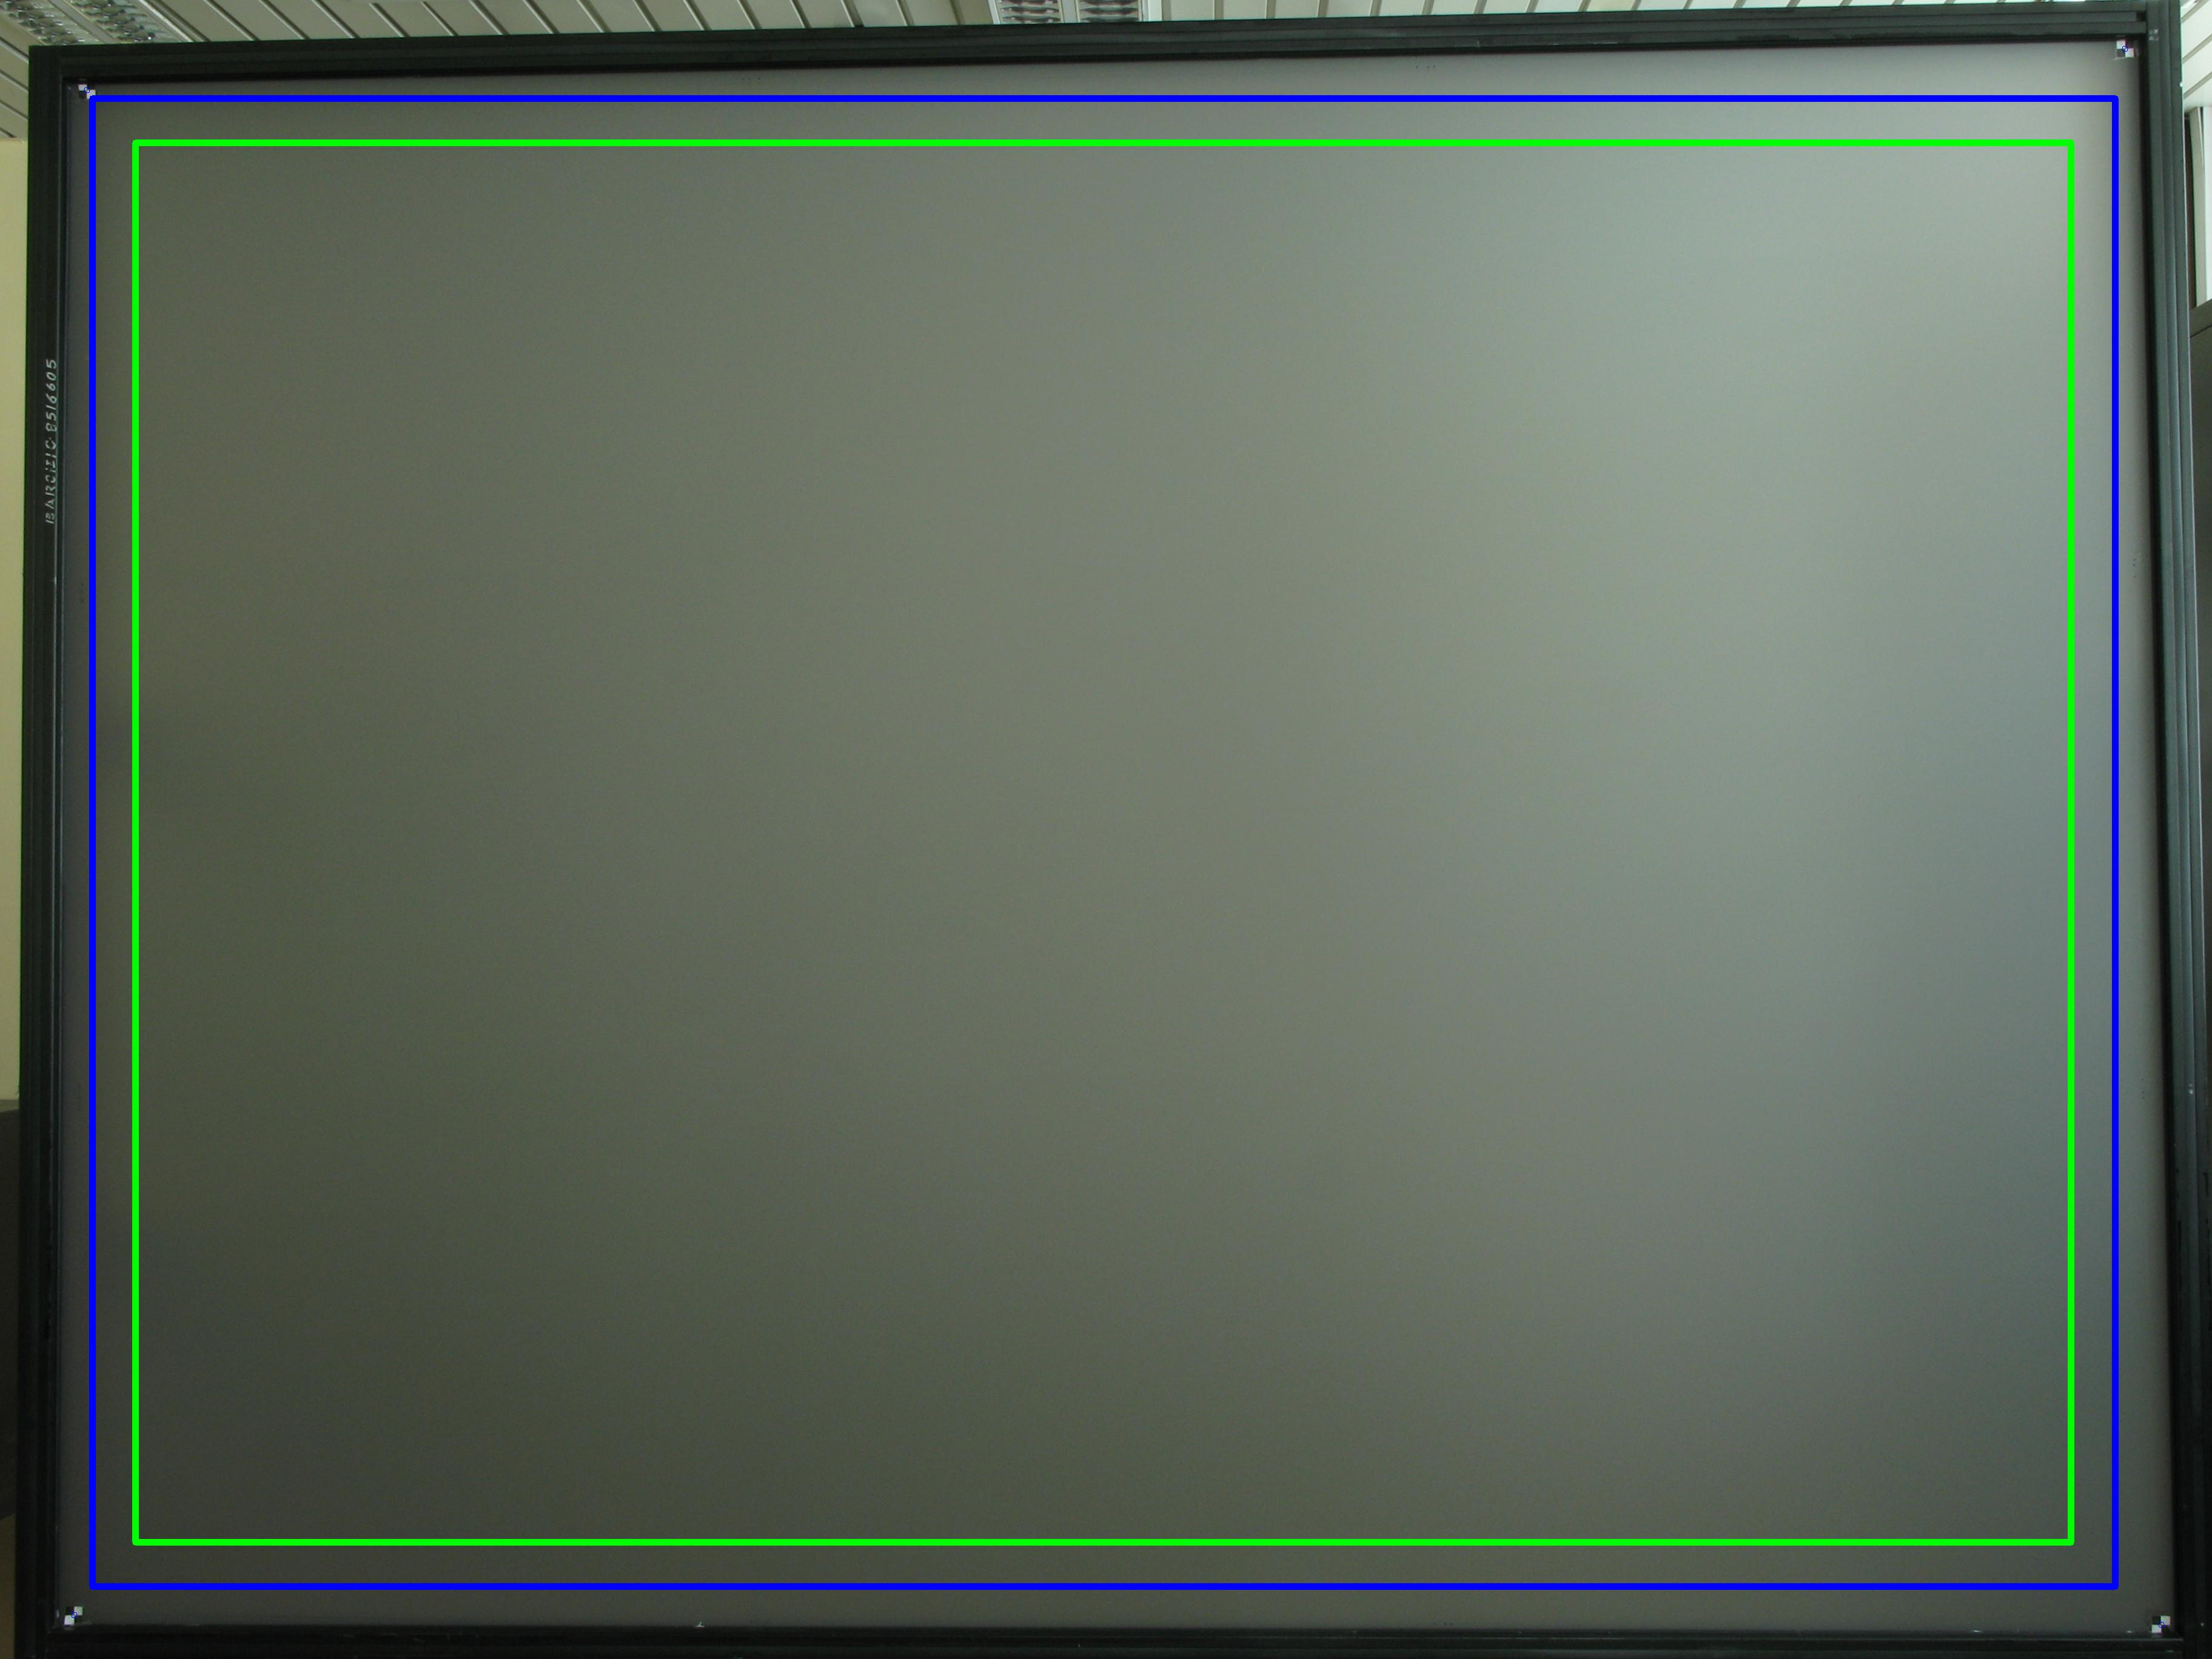
\includegraphics[width=5.0cm,height=4.0cm]{figures/crossratio_vs_noncrossratio.jpg}} \\
\end{tabular}
\end{tabularx}
\end{figure}


\end{frame}

%//////////////////////////////////////////////////////////////////////////////////////////////////////////////////////////////////
\section{Results}
\begin{frame}
\frametitle{Results\textsuperscript{\hyperlink{sysconfg}{*}}}
\begin{itemize}
\item Average misalignment between the grid lines projected at junction between neighbouring projectors was around $\sim1.0mm$ on a grid size of $\sim14$mm.
\begin{figure}
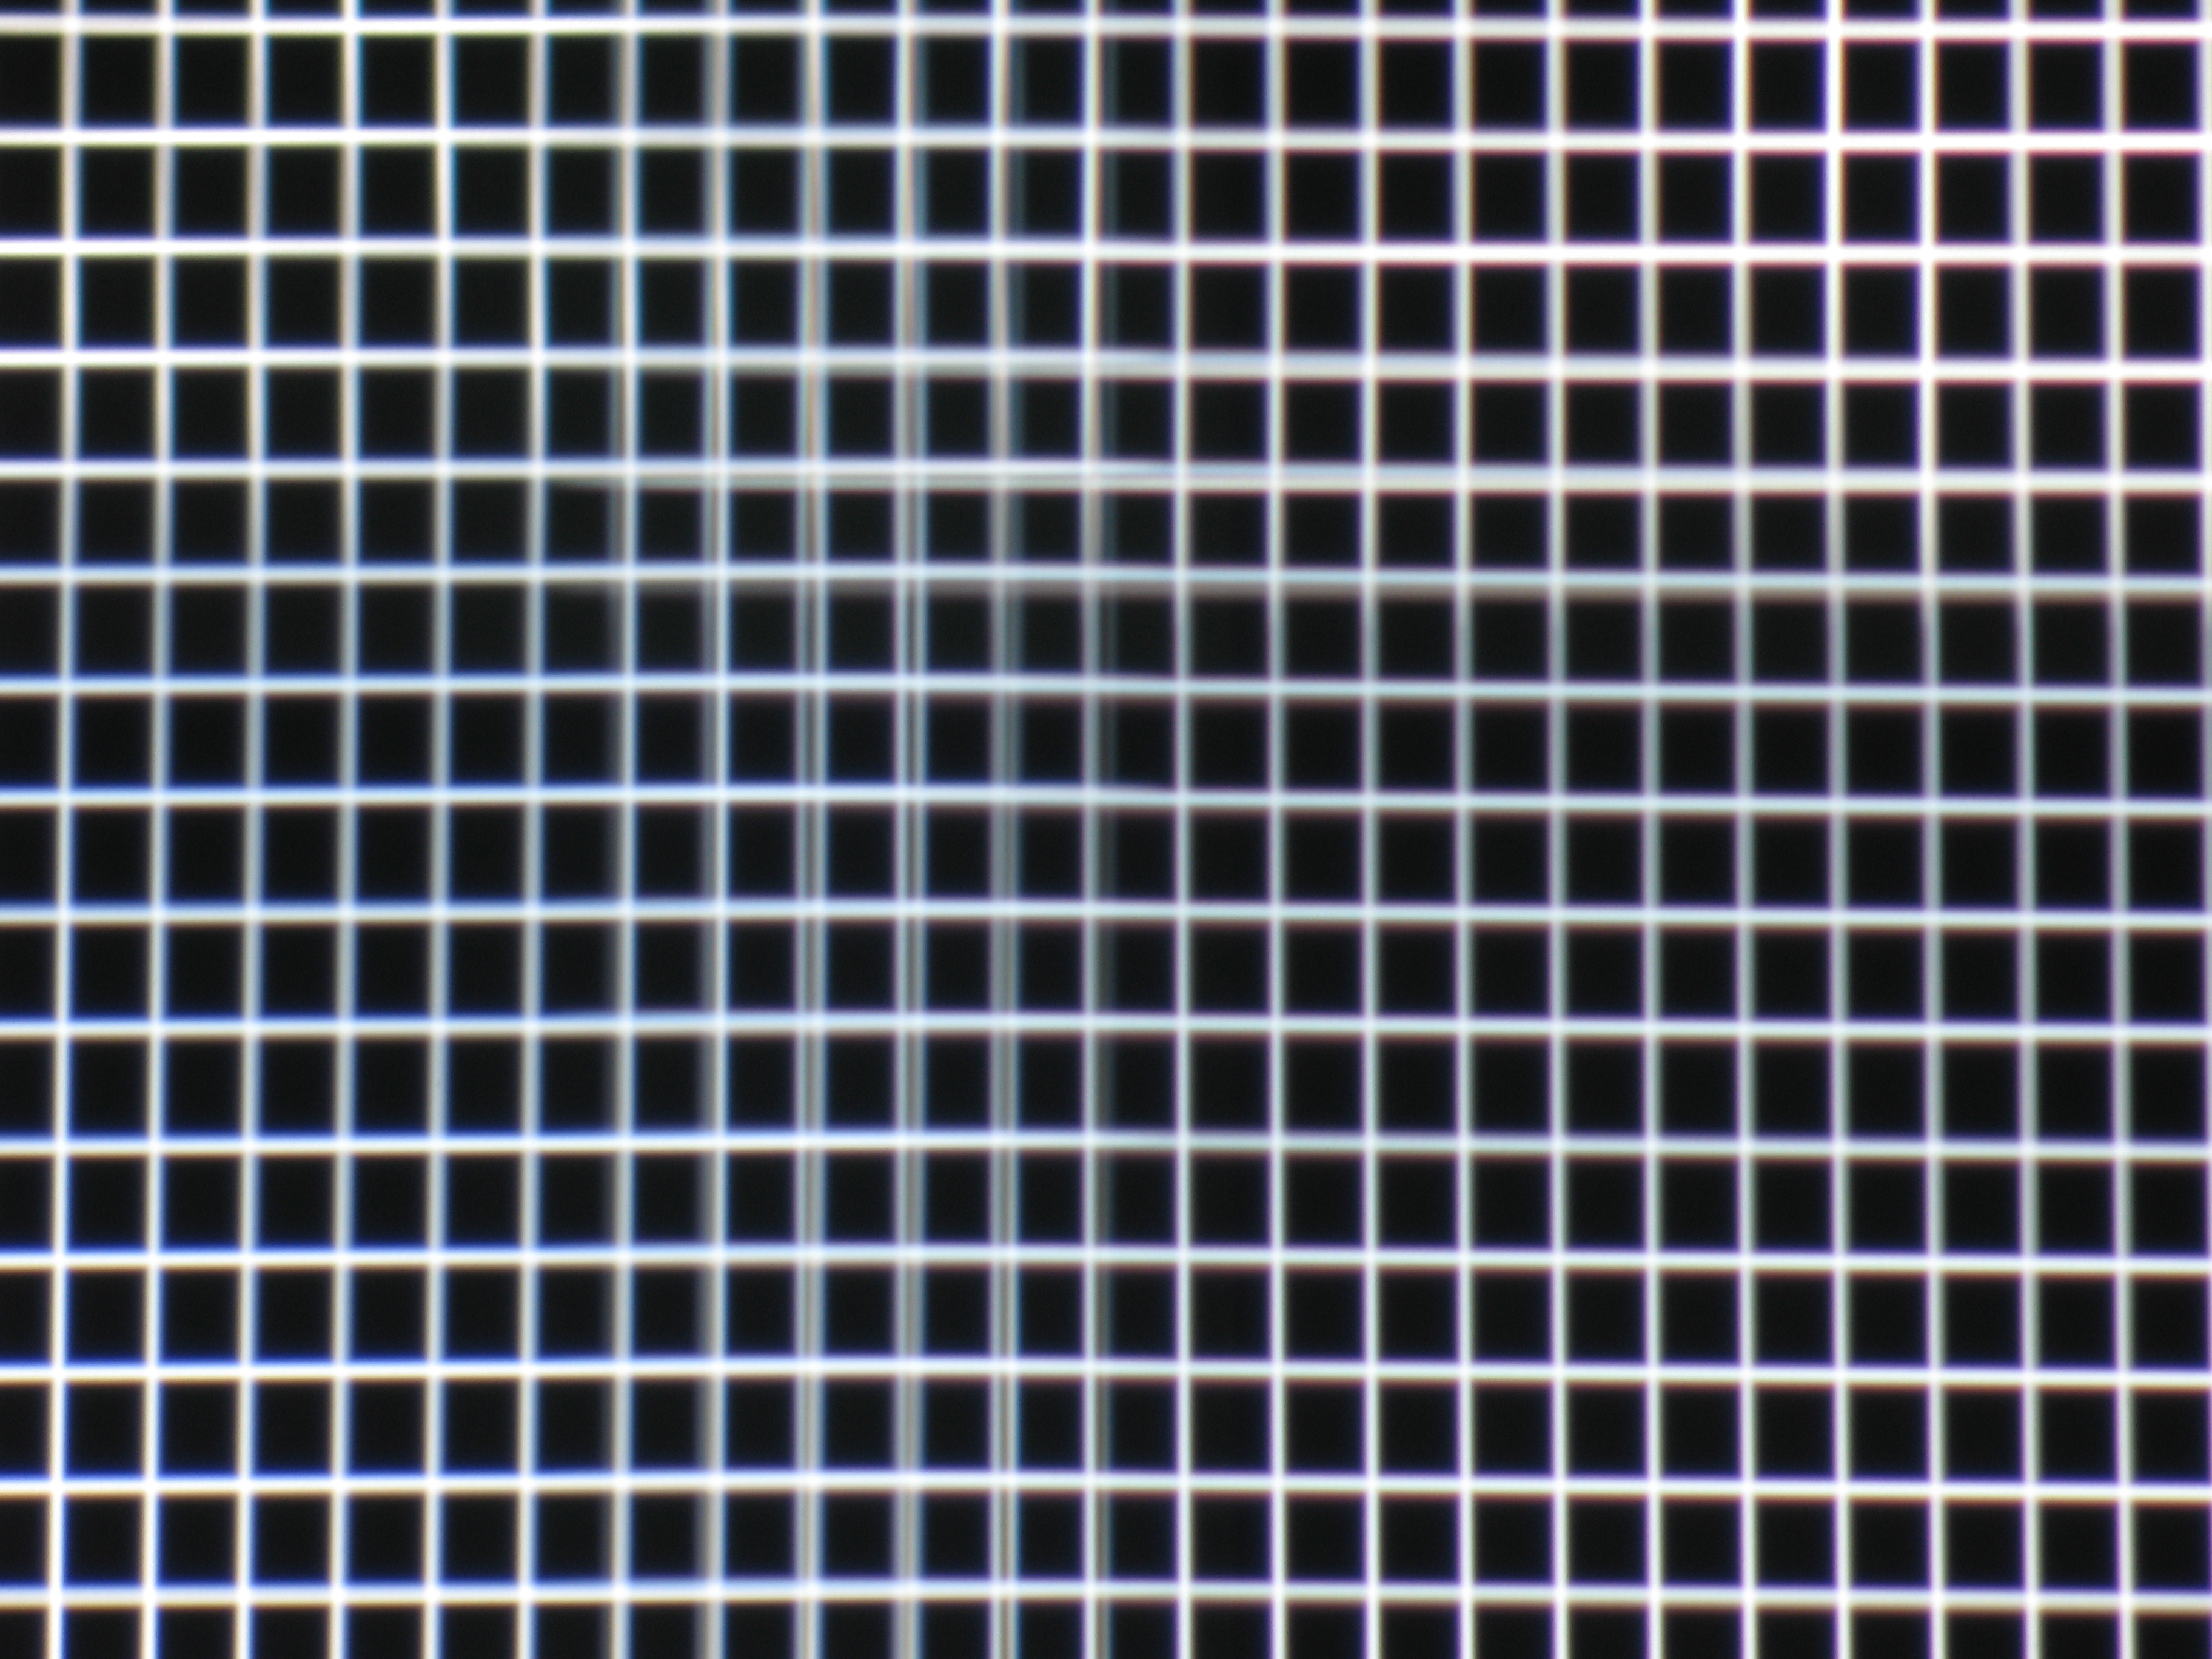
\includegraphics[width=6cm, height=4cm]{figures/grid.jpg}
\end{figure}
\end{itemize}
\end{frame}


\begin{frame}{Results(contd.)}
\begin{itemize}
\item Recovered $\sim10$\% more projection region using cross-ratio invariant.
\item Junctions between projectors are more imperceptible using cross ratio invariant.
\begin{figure}
\centering
\begin{tabularx}{\linewidth}{@{}cXX@{}}
\begin{tabular}{c c}
\hspace{0.5cm}\subfloat[Without cross ratio: seams more visible]{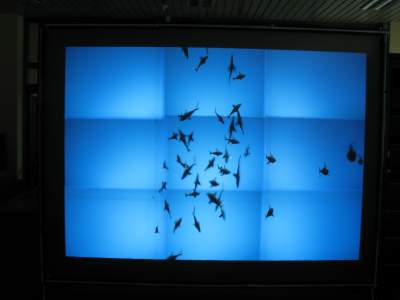
\includegraphics[width=4.0cm,height=3.0cm]{figures/without_cross_rat1.jpg}} &
\subfloat[With cross ratio: seams more imperceptible]{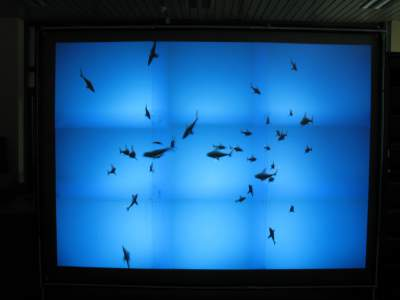
\includegraphics[width=4.0cm,height=3.0cm]{figures/with_cross_rat1.jpg}} \\
\end{tabular}
\end{tabularx}
\end{figure}

\item Resolution of the display is $\sim6.2$ Megapixels. 
\end{itemize}
\end{frame}

%//////////////////////////////////////////////////////////////////////////////////////////////////////////////////////////////////
\section{Conclusion}
\begin{frame}{Conclusion}

\begin{itemize}
\item Extension of the approach described in Brown's paper:
\begin{itemize}
\item Line-fitting 
\begin{itemize}
\item More uniform texture generation
\end{itemize}
\item Cross ratio:
\begin{itemize}
\item Full projection region 
\item Lesser imperceptible seams
\item Completely arbitrary placement of projectors
\end{itemize}
\end{itemize}

\item Limitations:
\begin{itemize}
\item Cross-ratio works only on planar surface
%\item Resolution\textsubscript{Utilzed} < Resolution\textsubscript{Native}
\item \texorpdfstring{Resolution\textsubscript{Utilized}}{Resolution Utilized} $<$ \texorpdfstring{Resolution\textsubscript{Native}}{Resolution Native}
%\item \texorpdfstring{like\textsubscript{this}}{like this}
\end{itemize}
\end{itemize}

\end{frame}
%//////////////////////////////////////////////////////////////////////////////////////////////////////////////////////////////////
\begin{frame}{Thank you!!}
\begin{figure}
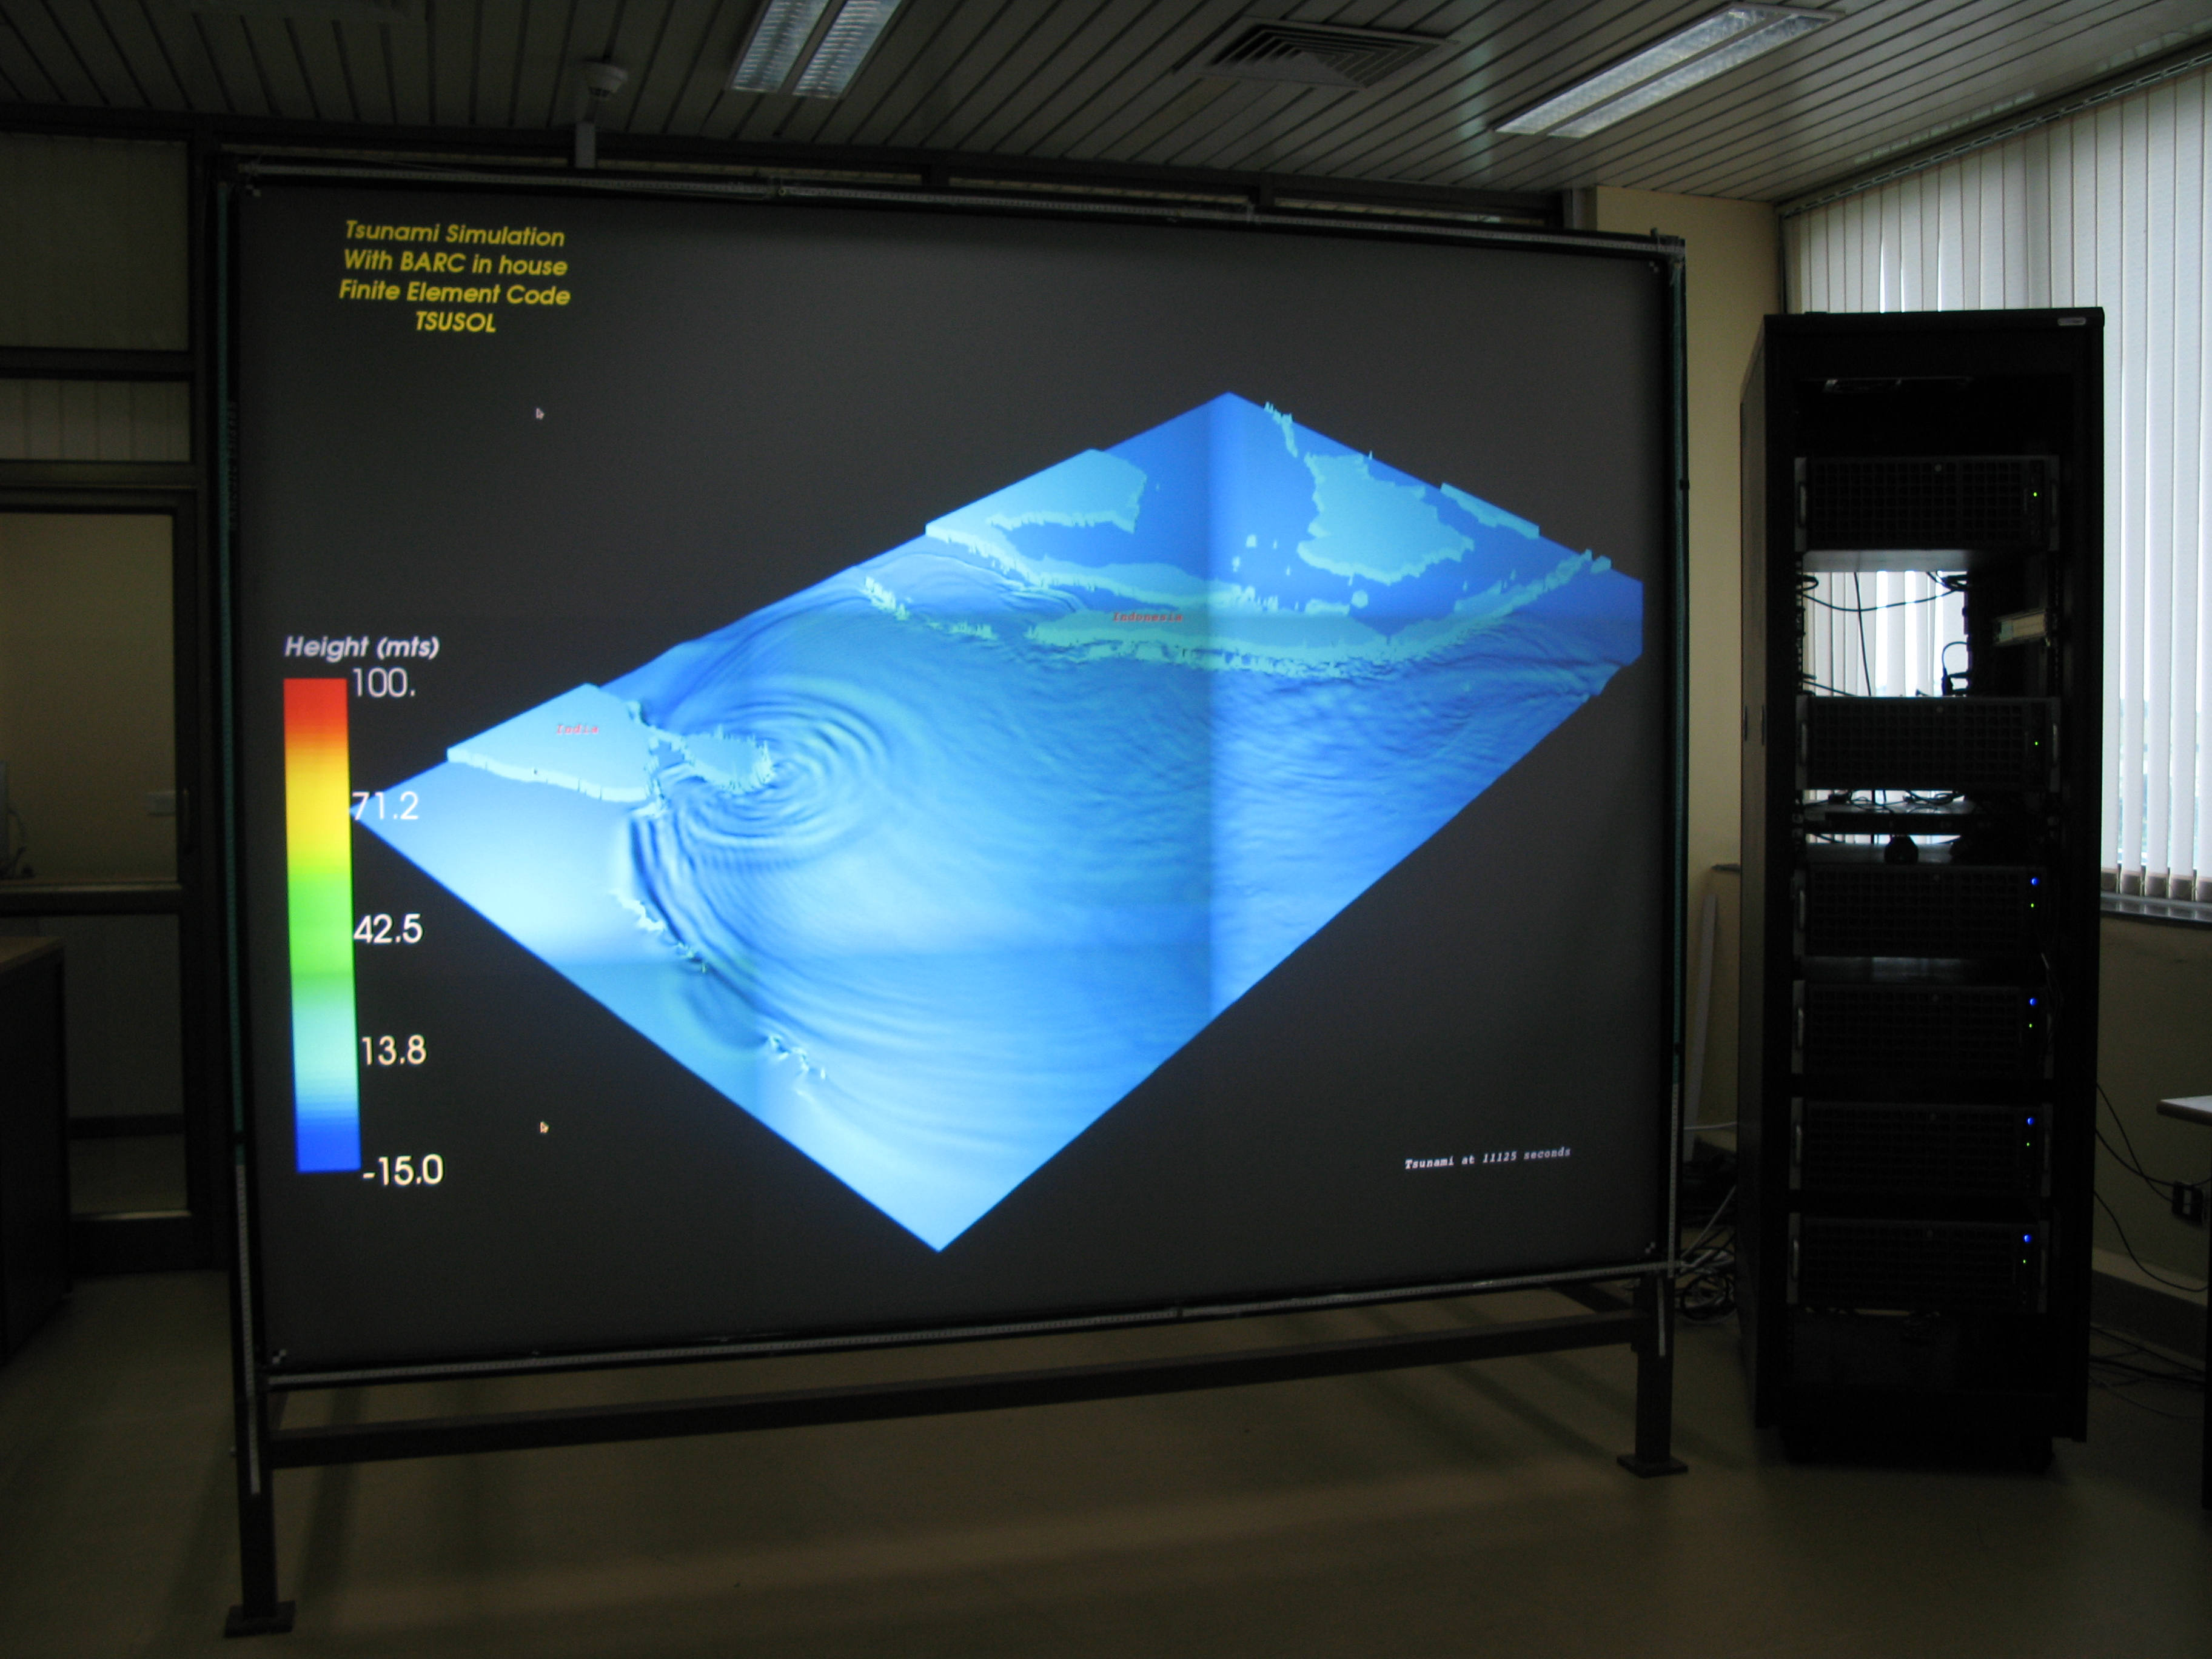
\includegraphics[width=\textwidth,height=\textheight]{figures/1.JPG}
\end{figure}
\end{frame}

%//////////////////////////////////////////////////////////////////////////////////////////////////////////////////////////////////

\appendix


%//////////////////////////////////////////////////////////////////////////////////////////////////////////////////////////////////
\begin{frame}[label=crossrat]
\frametitle{Cross ratio equations}
\begin{equation}
\begin{aligned}
x_t=B_c^x+t*(D_c^x-B_c^x)\\
y_t=B_c^y+t*(D_c^y-B_c^y)
\end{aligned}
\end{equation}

\begin{equation}
[t_1,t_2]=\frac{-b\pm\sqrt{b^{2}-4*a*c}}{2*a} 
\end{equation}
where,\newline
Let,\newline
$delta={CR_p*(\frac{|BC|_c}{|BD|_c})}^2$\newline
Then,
\begin{align*}
&a=(1-delta)*|BD|_c^2 \\
&b=2*{(D_c^x-B_c^x)*(B_c^x-C_c^x)+(D_c^y-B_c^y)*(B_c^y-C_c^y)}\\& \hspace{6cm}+2*|BD|_c^{2}*delta \\
&c=|BC|_c^2-delta*|BD|_c^2
\end{align*}




\end{frame}

%//////////////////////////////////////////////////////////////////////////////////////////////////////////////////////////////////

\begin{frame}[label=distform]
\frametitle{Edge blending equations}
\begin{itemize}
\item Distance transform:
\begin{equation}
\alpha(p,x_p,y_p)=\frac{d_p(x_p,y_p)}{\sum\nolimits_{i \in shares(i,x_g,y_g)} d_i(x_i,y_i)}
\end{equation}
\item Gamma correction:
\begin{equation}
\alpha(p,x_p,y_p)_\gamma=\alpha(p,x_p,y_p)^{\frac{1}{\gamma(p(x_p,y_p))}}
\end{equation}
\end{itemize}

\end{frame}

%//////////////////////////////////////////////////////////////////////////////////////////////////////////////////////////////////

\begin{frame}[label=sysconfg]
\frametitle{Experiment setup}
\begin{itemize}
\item \underline{Software}:
\begin{itemize}
\item Written in C
\item Dependent on OpenCV(v2.4.1) and libgphoto2(v2.5.2)
\item Works on Ubuntu(12.04 LTS) and Scientific Linux(6.1)
\end{itemize}      
\item \underline{Hardware}:
\begin{itemize}
\item 3X3 grid of NEC 200X DLP projectors
\item 2.4mX1.8m acrylic glass based rear projection screen(from ScreenTech,Germany)
\item Canon Powershot G7 digital camera
\item 4 Workstations(1 master+ 3 slave) each with Intel® Xeon® Six Core Processor X5670, NVIDIA Quadro FX 4600 Graphics card and 48 GB ECC RAM.
\end{itemize}
\end{itemize}
\end{frame}

%//////////////////////////////////////////////////////////////////////////////////////////////////////////////////////////////////



\end{document}

